\documentclass[12pt,oneside,a4paper]{book}
\usepackage{amsmath,amsthm,amssymb}
\usepackage{graphicx,float}
\usepackage{enumitem}
\usepackage[cm]{fullpage}
\usepackage{hyperref}
\usepackage{lmodern}
\usepackage{tikz}
\usetikzlibrary{positioning}
\hypersetup{
    colorlinks,
    citecolor=black,
    filecolor=black,
    linkcolor=blue,
    urlcolor=black
}

\theoremstyle{remark}
\newtheorem* {rem}{Remark}


\newtheorem{thm}{Theorem}[section]
\newtheorem{cor}[thm]{Corollary}
\theoremstyle{definition}
\newtheorem{prob}{Problem}[section]
\newtheorem{defn}{Definition}
\newtheorem*{ex}{Example}
\newtheorem*{soln}{Solution}

\newcommand{\ptoq}{p \to q}
\newcommand{\px}{P(x)}
\newcommand{\s}{\space}
\newcommand{\set}[1]{\left\{#1\right\}}
\begin{document}
\title{Discrete Math}
\author{Mehedi Hasan}
\maketitle
\newpage
\section*{Preface}
This is a compilation of lecture notes with some books and my own thoughts. This document is not a holy text. So, if there is a mistake, solve it by your own judgement.
\pagenumbering{roman}
\newpage
\tableofcontents
\newpage
\pagenumbering{arabic}
\part{Note}
\chapter{Logic and Proof}
\section{Proposition}
\begin{defn}[Proposition]
    A proposition is a declarative sentence (that is a sentence that declares a fact) that is either true or false but not both.
\end{defn}
\begin{ex}
    \hfill
    \begin{enumerate}
        \item Toronto is the capital of Canada.
        \item \(1+1=2\)
        \item $2+2=3$
    \end{enumerate}
    Proposition 1 and 3 are false where as 2 is true.\\
    Consider the following sentences:
    \begin{enumerate}
        \item What time it is?
        \item $x+y=z$
    \end{enumerate}
    are not propositions.
\end{ex}
\begin{defn}[Negation of $ p $]
    Let $p$ be a proposition.
    The negation of $p$ denoted by $\neg\ p$ (also denoted by $\bar{p}$) is the statement "It is not the case that p".
    The proposition $\neg\ p$ is read "not $p$".
\end{defn}
"Today is friday". \\
The negation is, "It is not the case that today is friday."
Simply, "Today is not friday."
\begin{table}[H]
    \centering
    \begin{tabular}{|c|c|}
        \hline
        p & \(\neg\ p\) \\ \hline
        T & F           \\ \hline
        F & T           \\ \hline
    \end{tabular}
    \caption{Truth table for negation of a proposition}
\end{table}
\begin{defn}[Conjunction of \(p\) and \(q\)]
    Let \(p\) and \(q\) be propositions. The conjunction of \(p\) and \(q\), denoted by \((p\wedge q)\) is the proposition "p and q". The conjunction \(p\wedge q\) is true when both \(p\) and \(q\) are true and is false otherwise.
\end{defn}
"Today is friday and it is raining."

\begin{table}[H]
    \centering
    \begin{tabular}{|c|c|c|}
        \hline
        p & q & \(p\wedge q\) \\ \hline
        T & T & T             \\ \hline
        T & F & F             \\ \hline
        F & T & F             \\ \hline
        F & F & F             \\ \hline
    \end{tabular}
    \caption{Truth table for \(p\wedge q\)}
\end{table}
\begin{defn}[Disjunction of \(p\) and \(q\)]
    Let \(p\) and \(q\) be propositions. The disjunction of \(p\) and \(q\) denoted by \((p \vee q)\) is the proposition "p or q". The disjunction \(p\vee q\) is false when both \(p\) and \(q\) are false and is true otherwise.
\end{defn}
"Students who have taken calculus or computer science can take this class."
\begin{table}[H]
    \centering
    \begin{tabular}{|c|c|c|}
        \hline
        p & q & \(p\vee q\) \\ \hline
        T & T & T           \\ \hline
        T & F & T           \\ \hline
        F & T & T           \\ \hline
        F & F & F           \\ \hline
    \end{tabular}
    \caption{Truth table for \(p\vee q\)}
\end{table}
\begin{defn}[Exclusive or of \(p\) and \(q\)]
    Let \(p\) and \(q\) be propositions. The exclusive or of \(p\) and \(q\) denoted by \((p \oplus q)\) is the proposition that is true when exactly one of \(p\) and \(q\) is true and is false otherwise.
\end{defn}
"Students who have taken calculus or computer science, but not both, can take this class."
\begin{table}[H]
    \centering
    \begin{tabular}{|c|c|c|}
        \hline
        p & q & \(p\oplus q\) \\ \hline
        T & T & F             \\ \hline
        T & F & T             \\ \hline
        F & T & T             \\ \hline
        F & F & F             \\ \hline
    \end{tabular}
    \caption{Truth table for \(p\oplus q\)}
\end{table}
Let \(p\) and \(q\) be propositions. The conditional statement \(p \to q\) is the proposition "If p then q". The conditional statement \(p\to q\) is false when \(p\) is true and \(q\) is false and true otherwise. In the conditional statement \(p\to q\), \(p\) is called hypothesis and \(q\) is called conclusion.
"If I am elected, then I will lower taxes."
\begin{table}[H]
    \centering
    \begin{tabular}{|c|c|c|}
        \hline
        p & q & \(p\to q\) \\ \hline
        T & T & T          \\ \hline
        T & F & F          \\ \hline
        F & T & T          \\ \hline
        F & F & T          \\ \hline
    \end{tabular}
    \caption{Truth table for \(p\to q\)}
\end{table}
\begin{defn}[Converse, Contrapositive and Inverse]
    The proposition \(q\to p\) is called converse of \(\ptoq\).
    The contrapositive of \(\ptoq\) is the proposition \(\neg\ q \to \neg\ p\).
    The proposition \(\neg\ p \to \neg\ q\) is called inverse of \(\ptoq\).
\end{defn}
\begin{ex}
    "If it is raining, then the home team wins."\\
    Contrapositive: If the home team does not win then it is not raining.\\
    Converse: If the home team wins, then it is raining.\\
    Inverse: If it is not raining, then the home  team does not win.
\end{ex}
\begin{defn}[Biconditional]
    Let $ p $ and $ q $ be propositions. The biconditional statement \(p\leftrightarrow q\) is the proposition "p if and only if q". The biconditional statement \(p\leftrightarrow q\) is true when $ p $ and $ q $ have the same truth values and is false otherwise.
    "You can take the flight if and only if you buy a ticket."
    \[(\ptoq)\wedge(q\to p)\]
\end{defn}

\begin{table}[H]
    \centering
    \begin{tabular}{|c|c|c|}
        \hline
        p & q & \(p\leftrightarrow q\) \\ \hline
        T & T & T                      \\ \hline
        T & F & F                      \\ \hline
        F & T & F                      \\ \hline
        F & F & T                      \\ \hline
    \end{tabular}
    \caption{Truth table for \(p\leftrightarrow q\)}
\end{table}
\begin{prob}
    Construct the truth table of the compound proposition.\[(p\vee \neg\ q)\to (p\wedge q)\]
\end{prob}
\begin{soln}
    Let us construct a table
    \begin{center}
        \begin{tabular}{|c|c|c|c|c|c|}
            \hline
            $ p $ & $ q $ & \(\neg\ q\) & \(p\vee \neg\ q\) & \(p \wedge q\) & \((p\vee \neg\ q)\to (p\wedge q)\) \\ \hline
            T     & T     & F           & T                 & T              & T                                  \\ \hline
            T     & F     & T           & T                 & F              & F                                  \\ \hline
            F     & T     & F           & F                 & F              & T                                  \\ \hline
            F     & F     & T           & T                 & F              & F                                  \\ \hline
        \end{tabular}
    \end{center}
\end{soln}
\begin{prob}
    How can this English sentence be translated into a logical expression?\\
    "You can access the internet from campus only if you are a computer science major or you are not a freshman."
\end{prob}
\begin{soln}
    \hfill\\
    \indent$ a $ \(\to\) You can access the internet from campus\\
    \indent$ b $ \(\to\) You are a computer science major\\
    \indent$ c $ \(\to\) You are a freshman\\
    \indent\(a\to(b\vee\neg\ c)\)
\end{soln}
\begin{itemize}
    \item Computer represent information using bits.
    \item A bit is a symbol with two possible values, namely, 0 and 1, 1 represents true, 0 represents false.
    \item A variable is called a Boolean variable if its value is either true or false.
    \item A bit string is a sequence of zero or more bits. The length of this string is the number of bits in this string.
          \begin{align*}
              01\,1011\,0110   &                                   \\
              11\, 0001 \,1101 &                                   \\\cline{1-1}
              11 \,10111\, 111 & \longleftarrow \text{bitwise OR}  \\
              01 \,0001 \,0100 & \longleftarrow \text{bitwise AND} \\
              10 \,1010\, 1011 & \longleftarrow \text{bitwise XOR}
          \end{align*}
\end{itemize}
\begin{defn}[Tautology and Contradiction]
    A compound proposition that is always true, no matter what the truth values of the propositions that occur in it is called tautology.
    A compound proposition that is always false is called a contradiction.
    A compound proposition that is neither a tautology nor a contradiction is called a contingency.
\end{defn}
\begin{table}[H]
    \centering
    \begin{tabular}{|c|c|c|c|}
        \hline
        $ p $ & \(\neg\ p\) & \(p\wedge \neg\ p\) & \(p\vee\neg\ p\) \\ \hline
        T     & F           & F                   & T                \\ \hline
        F     & T           & F                   & T                \\ \hline
    \end{tabular}
    \caption{Truth table for tautology and contradiction}
\end{table}
\begin{defn}[Logically Equivalent]
    The compound proposition $ p $ and $ q $ are called logically equivalent if \(p\leftrightarrow q\) is a tautology. It is denoted as \(p \equiv q\)
\end{defn}
\begin{table}[H]
    \centering
    \begin{tabular}{|c|c|c|c|c|c|c|}
        \hline
        $ p $ & $ q $ & \(p\vee q\) & \((\neg\ p\vee q)\) & \(\neg\ p\) & \(\neg\ q\) & \(\neg\ p\wedge \neg\ q\) \\ \hline
        T     & T     & T           & F                   & F           & F           & F                         \\ \hline
        T     & F     & T           & F                   & F           & T           & F                         \\ \hline
        F     & T     & T           & F                   & T           & F           & F                         \\ \hline
        F     & F     & F           & T                   & T           & T           & T                         \\ \hline
    \end{tabular}
    \caption{Truth table for logically equivalent}
    \[(\neg\ p\vee q)\equiv \neg\ p\wedge \neg\ q\]
\end{table}
\begin{prob}
    Prove that \(p\vee(q\wedge r)=(p\vee q)\wedge(p\vee r)\)
\end{prob}
\begin{prob}
    Show that \((\neg\ p\vee(\neg\ p\wedge q))\equiv\neg\ p \wedge \neg\ q\)
\end{prob}
\begin{soln}
    \begin{align*}
        \neg\ (p\vee(\neg\ p\wedge q)) & \equiv \neg\ p \wedge \neg\ (\neg\ p \wedge q)       \\
                                       & \equiv \neg\ p \wedge (\neg\ \neg\ p\vee \neg\ q)    \\
                                       & \equiv \neg\ p \wedge(p\vee \neg\ q)                 \\
                                       & \equiv (\neg\ p\wedge p) \vee (\neg\ p \vee \neg\ q) \\
                                       & \equiv \neg\ p \vee \neg\ q
    \end{align*}
\end{soln}
\begin{defn}[Predicates]
    Suppose a statement involving variables, such as \(x>3\)\\
    The statement "x is greater than 3" has two parts.
    The first part, the variable $ x $, is the subject of the statement.
    The second part - the predicate, "is greater than 3" refers to a property that the subject of the statement can have.

    We can denote the statement by \(P(x)\), where $ p $ denotes the predicates and x is the variable.
    Propositional function p at x. Once a value has been assigned to the variable $ x $ the statement \(P(x)\) becomes a proposition and has a truth value.
\end{defn}
\begin{ex}
    Let \(P(x)\) denotes the statement "\(x>3\)". What are the values of \(P(4)\) and \(P(2)\)?\\
    \(P(4)\), which is the statement "\(4>3\)" is true and \(P(2)\), which is the statement "\(2>3\)" is false.
\end{ex}
A statement of the form \(P(x_1,x_2,\dot,x_n)\) is the value of the propositional function $ P $ at the n-tuple \((x_1,x_2,\dot,x_n)\) and $ P $ is called an n-place predicate or a n-ary predicate.
\begin{prob}
    Consider the following program:
    \begin{quote}
        temp:=x\\x:=y\\y:=temp
    \end{quote}
    Find predicates that we can use as the precondition and the post-condition to verify the correctness of this program.
    Then explain how to use them to verify that for all valid input the program does what is intended?
\end{prob}
TODO:: Solve this.
\begin{defn}[Quantifiers]
    The universal quantification of \(P(x)\) is the statement "\(P(x)\) for all the values of x in the domain".
    THe notation \(\forall x P(x)\) denotes the universal quantification of \(P(x)\) and \(\forall\) is called the universal quantifier.

    An element for which \(P(x)\) is false is called a counterexample of \(\forall x P(x)\).
\end{defn}
\begin{ex}
    Let \(P(x)\) be the statement "\(x+1>x\)". What is the truth value of the quantification \(\forall x P(x)\). Where domain consists of all real numbers?

    Because \(P(x)\) is true for all real numbers \(x\), the quantification, \(\forall x P(x)\) is true.
\end{ex}
\begin{defn}[Existential Quantifier]
    The existential quantification of \(P(x)\) is the proposition "There exists an element $ x $ in the domain such that \(P(x)\)."

    We use the notation \(\exists xP(x)\) for the existential quantification of \(P(x)\). Here \(\exists\) is called the existential quantifier.
    Let \(P(x)\) denote the statement "\(x>3\)". What is the truth value of the quantification \(\exists xP(x)\), where the domain consists of all real numbers?
\end{defn}
\paragraph{\#}\(\forall x<0\,(x^2>0)\), \(\forall y\neq 0(y^3\neq 0)\)\\
\(\forall x (x<0 \rightarrow x^2>0)\) \(\forall y (y\neq 0\rightarrow y^3\neq0)\)\\
\(\exists z>0(z^2=2)\)\\\(\exists z (z>0\wedge z^2=2)\)
\paragraph{\#} Statements involving predicate and quantifiers are logically equivalent if and only if they have the same truth value no matter which predicates are substituted into these statement and which domain of discourse is used for the variables in these propositional function.
\begin{prob}
    Show that \(\forall x\,(P(x)\wedge Q(x))\) and \(\forall x\,P(x)\wedge \forall x\,Q(x)\) are logically equivalent.
\end{prob}
\begin{soln}
    Let \(\forall x\,(P(x)\wedge Q(x))\) is true. This means if $ a $ is in the domain then \((P(a)\wedge Q(a))\) is true. Hence \(P(a)\) and \(Q(a)\) is true for every element in the domain, we can conclude that \(\forall xP(x)\) and \(\forall xQ(x)\) are both true. This means that \(\forall xP(x)\wedge\forall x Q(x)\) is true.

    Next suppose that \(\forall xP(x)\wedge\forall x Q(x)\) is true. It follows that \(\forall xP(x)\) is true and \(\forall xQ(x)\) is true.
    Hence if $ a $ is in the domain, \(P(a)\) is true and \(Q(a)\) is true. It follows that for all $ a $, \(P(a)\wedge  Q(a)\) is true. Hence \(\forall x(P(x)\wedge Q(x))\) is true.
\end{soln}
\(\neg\ \forall\ xP(x)\equiv\exists\ x\neg\ P(x)\)
\begin{enumerate}
    \item \( \neg\ \exists x \px \equiv \forall x \neg\ \px\) [For every $ x $, $ \px $ is false]
    \item \(\neg\ \forall x\px \equiv\exists x\neg\px\) [There is an $ x $ for which $ \px $ is false]
\end{enumerate}
\begin{prob}
    Show that, \(\neg\ \forall x(\px\to Q(x))\equiv\exists x(\px\wedge\neg\ Q(x))\)
\end{prob}
TODO: solve Problem
\begin{prob}
    Express the statements "some student in this class has visited Mexico" and "Every student in this class has visited either Canada or Mexico" using predicates and quantifiers.
\end{prob}
\begin{soln}
    Let,\\
    \(S(x)\to x\) is a student in this class.\\
    \(M(x)\to x\) has visited Mexico.\\
    \(C(x)\to x\) has visited Canada.\\
    The solution for first statement is \(\exists x (S(x)\wedge M(x))\)\\
    The solution for second statement is \(\forall x (S(x)\to (C(x)\vee M(x)))\)
\end{soln}
\begin{defn}[Theorem]
    A theorem is a statement that can be shown to be true.
    Less important theorems sometimes are called \emph{proposition}.
\end{defn}
\begin{defn}[Proof]
    A proof is a valid argument that establish the truth of a theorem.
\end{defn}
\begin{defn}[Lemma]
    A less important theorem that is helpful in proof of other results is called a lemma.
\end{defn}
\begin{defn}[Corollary]
    A corollary is a theorem that can be established directly from a theorem that has been proved.
\end{defn}
\begin{defn}[Conjucture]
    A conjecture is a statement that is being proposed to be true statement, usually on the basis of some partial evidence.
\end{defn}
\begin{defn}[Direct Proof]
    A direct proof of a conditional statement \(\ptoq\) is constructed when the first step is the assumption that $ P $ is true; subsequent steps are constructed using rules of interference, with the final step showing that \(q\) must also be true.
\end{defn}
\begin{defn}[Indirect Proof]
    The proof that do not start with the hypothesis and end with the conclusion are called indirect proof.
\end{defn}
\begin{defn}[Proof by Contraposition]
    Proof by contraposition means that the conditional statement \(\ptoq\) can be proved by showing that the contrapositive \(\neg\ q\to\neg\ p\) is true.
\end{defn}
\begin{prob}
    Prove that if \(n\) is an integer and \(3n+2\) is odd, then \(n\) is odd.
\end{prob}
\begin{proof}
    Direct proof:

    Let, \(3n+2\) is odd and \(3n+2=2k+1\), for some integer \(k\)\\
    This implies, \(3n+1=2k\)\\
    There does not seem to be any direct way to conclude that \(n\) is odd.

    Our attempt at direct proof failed.

    Proof by contraposition:

    Assume that \(n\) is even.\\
    So, \(n=2k\) for some integer \(k\).\\
    So, we have,
    \[3n+2=3(2k)+2=2(3k+1)\]
    This tells us that \(3n+2\) is even.

    Because the negation of the conclusion of the conditional statement implies that the hypothesis is false, the original conditional statement is true.
\end{proof}
\begin{defn}[Vacuous Proof]
    \(\ptoq\) is true when $ P $ is false \(\ptoq\equiv(\neg\ p\vee q)\).\\ If we can show that $ p $ is false, then we have a proof called a vacuous proof of the conditional statement \(\ptoq\).
\end{defn}
\begin{defn}[Trivial Proof]
    A proof of \(\ptoq\) that uses the fact that $ q $ is true is called a trivial proof.
\end{defn}
\begin{defn}[Proofs by Contradiction]
    Because the statement \(r\wedge\ \neg\ r\) is a contradiction whenever $ r $ is a proposition, we can prove that $ p $ is true if we can show that \(\neg\ p\to(r\wedge\ \neg\ r)\) is true for some proposition $ r $. Proofs of this type are called proofs by contradiction.
\end{defn}
\begin{prob}
    Prove that \(\sqrt{2}\) is irrational by giving a proof by contradiction.
\end{prob}
\begin{proof}
    If \(\sqrt{2}\) is rational, there exists integer \(a\) and \(b\) with, \(\sqrt{2}=\frac{a}{b}\) where $ a $ and $ b $ have no common factors.(Every rational number can be written in lowest terms.)
    So, \(2=\frac{a^2}{b^2}\Rightarrow2b^2=a^2\) \\
    So, \(a^2\) is even and $ a $ is also even.\\
    So, \(a=2c\). Then, \(2b^2=4c^2\Rightarrow b^2=2c^2\)\\
    Similarly $ b $ is also even.\\
    Now we have $ a $ and $ b $ have no common factors, $ a $ ans $ b $ are even, that is 2 divides both $ a $ and $ b $.

    Because our assumption of \(\neg\ p\) leads to the contradiction that 2 divides both $ a $ and $ b $ and 2 does not divide both $ a $ and $ b $, \(\neg\ p\) must be false.\\
    So \(\sqrt2\) must be irrational.
\end{proof}
A statement of the form \(\forall x\px\) is false we need only find a counterexample that is an example for which \(\px\) is false.

Mistakes is proofs:
\begin{align*}
                & \,a = b              \\
    \Rightarrow & \,a^2 =ab            \\
    \Rightarrow & \,a^2-b^2=ab-b^2     \\
    \Rightarrow & \,(a+b)(a-b)= b(a-b) \\
    \Rightarrow & \,a+b=b              \\
    \Rightarrow & \,2b=b               \\
    \Rightarrow & \,2=1
\end{align*}
\begin{defn}[Exhaustive Proof]
    Some theorems can be proved by examining a relatively small number of examples. Such proofs are called exhaustive proof.
\end{defn}
\begin{ex}
    Prove that, \((n+1)^3\geq3^n\) if n is a positive integer and \(n\leq4\).\\
    If \(n=1,\quad(1+1)^3\geq3^1\,\Rightarrow8\geq3\)\\
    \(n=2,\quad(2+1)^3\geq3^2\,\Rightarrow27\geq9\)\\
    \(n=3,\quad(3+1)^3\geq3^3\,\Rightarrow64\geq27\)\\
    \(n=4,\quad(4+1)^3\geq4^3\,\Rightarrow125\geq81\)\\
\end{ex}
A proof by cases must cover all possible cases that arise in a theorem.\\
When the phrase "without loss of generality" is used in a proof, we assert that by proving one case of a theorem, no additional argument is required to prove other specified cases.
\begin{defn}[Uniqueness Proofs]
    The two parts of a uniqueness proof are:
    \begin{itemize}
        \item \textbf{Existence:} We show that an element $ x $ with desired property exists.
        \item \textbf{Uniqueness:} We show that if \(y\neq x\), then $ y $ does not have the desired property.\\
              Equivalently, we can show that if $ x $ and $ y $ both has the desired property, then \(x=y\).
    \end{itemize}
\end{defn}
\begin{defn}[Argument]
    By an argument, we mean a sequence of statements that end with a conclusion.\\
    By \emph{valid}, we mean that the conclusion or final statement of the argument must follow form the truth of the preceding statements or premises of the argument.

    That is an argument is valid if and only if it is impossible for all the premises to be true and the conclusion to be false.
\end{defn}
\begin{defn}[Premises \& Conclusion]
    An argument in propositional logic is a sequence of propositions. All but the final proposition in the argument are called premises and the final proposition is called the conclusion.

    An argument is valid if the truth of all its premises implies that the conclusion is true.
\end{defn}
\paragraph{\#}
We can first establish the validity of some relatively simple argument forms called rules of interference.\\
\(p\to\) It is below freezing now\\
\(q\to\) It is raining now\\
"It is below freezing now. Therefore it is either below freezing or raining now."\\
\begin{align*}
    p \qquad\qquad                   & p\to(p\vee q)\quad \text{addition} \\
    \cline{1-1}
    \therefore\, p \vee q \qquad\,\, &                                    \\
\end{align*}
\begin{table}[H]
    \centering
    \begin{tabular}{|c|c|c|}
        \hline
        Rule of interference             & Tautology                                                & Name                   \\\hline
        {\(\begin{aligned}
                p                       &         \\
                p                       & \to \ q \\
                \cline{1-2}\therefore q &
            \end{aligned}\)} & \([p\wedge(\ptoq)]\to q\)                                & Modus pones            \\\hline
        {\(\begin{aligned}
                \neg\ q                       &         \\
                p                             & \to \ q \\
                \cline{1-2}\therefore \neg\ p &
            \end{aligned}\)} & \([\neg\ q\wedge(\ptoq)]\to \neg\ q\)                    & Modus tollens          \\\hline
        {\(\begin{aligned}
                p                       & \to\ q  \\
                q                       & \to \ r \\
                \cline{1-2}\therefore p & \to\ r
            \end{aligned}\)} & \([(\ptoq)\wedge(q\to q)]\to (p\to r)\)                  & Hypothetical Syllogism \\\hline
        {\(\begin{aligned}
                p                       & \wedge\ q \\
                \neg\&p                             \\
                \cline{1-2}\therefore q &
            \end{aligned}\)} & \([(p\vee\ q)\wedge\neg\ p]\to q\)                       & Disjunctive Syllogism  \\\hline
        {\(\begin{aligned}
                p                       &         \\
                \cline{1-2}\therefore p & \vee\ q
            \end{aligned}\)} & \(p\to (p\vee\ q)\)                                      & Addition               \\\hline
        {\(\begin{aligned}
                p                       & \wedge\ q \\
                \cline{1-2}\therefore p &
            \end{aligned}\)} & \((p\wedge\ q)\to p\)                                    & Simplification         \\\hline
        {\(\begin{aligned}
                p                       &            \\
                q                       &            \\
                \cline{1-2}\therefore p & \wedge \ q
            \end{aligned}\)} & \([(p)\wedge (q)]\to (p\wedge\ q)\)                      & Conjunction            \\\hline
        {\(\begin{aligned}
                p                       & \vee\ q \\
                \neg                              \\ p &\vee \ r\\
                \cline{1-2}\therefore q & \vee\ r
            \end{aligned}\)} & \([(p\vee\ q)\ \wedge\ (\neg\ p \vee\ r)]\to (q\vee\ r\) & Resolution             \\\hline
    \end{tabular}
    \caption{Rules of Interference}
\end{table}
\begin{prob}
    Show that the hypothesis "It is not sunny this afternoon and it is colder than yesterday",
    "We will go swimming only if it is sunny",
    "If we do not go swimming, then we will take a canoe trip", and
    "If we take a canoe trip, then we will be home by sunset"
    lead to the conclusion "We will be home by sunset."
\end{prob}
\begin{soln}
    Let,\newline
    \(p\to\) It is sunny this afternoon\\
    \(q\to\) It is colder than yesterday\\
    \(r\to\) We will go swimming\\
    \(s\to\) We will take a canoe trip\\
    \(t\to\) We will be home by sunset\\

    We construct an argument to show that our hypothesis lead to the desired conclusion as follows:\\
    \begin{tabular}{p{.4\textwidth} p{.4\textwidth}}
        \qquad Steps & \qquad Reason              \\
        {
        \begin{enumerate}
            \item \(\neg\ p\wedge\ q\)
            \item \(\neg\ p\)
            \item \(r\to\ p\)
            \item \(\neg\ r\)
            \item \(\neg\ r\to s\)
            \item \(s\)
            \item \(s\to t\)
            \item \(t\)
        \end{enumerate}
        }            & \begin{itemize}
            \item [] Hypothesis
            \item [] Simplification using 1
            \item [] Hypothesis
            \item [] Modus tollens using 2 and 3
            \item [] Hypothesis
            \item [] Modus pones using 4 and 5
            \item [] Hypothesis
            \item [] Modus pones using 6 and 7
        \end{itemize} \\
    \end{tabular}
\end{soln}
\begin{prob}
    Prove that, if $ n $ is an integer then \(n^2\geq\ n\).
\end{prob}
\begin{proof}
    We split the proof into three cases.\\
    Case i: When \(n=0\), because \(0^2=0\). We see that, \(0^2=0\).
    It follows that \(n^2\geq\ n\) is true in this case.\\
    Case ii: When \(n\geq\ 1\). We obtain \(n^2\geq\ n\) for positive integer n.\\
    Case iii: When \(n\leq\ -1\). We obtain \(n^2\geq\ 0\geq\ n\)

    Because the inequality \(n^2\geq\ n\) holds in all three cases, we can conclude that if n is an integer then \(n^2\geq\ n\).
\end{proof}
\paragraph{\# Division Algorithm} Let $ a $ be an integer and $ d $ be a positive integer.
Then there are unique integers $ q $ and $ r $ with \(0\geq\ r <\ d\).
Such that,
\[a=\ dq+r\]
\[q=\ \text{div}\ d,\qquad r=\ a \mod \ d\]
\begin{prob}
    What are the quotients when -11 is divided by 3?
\end{prob}
\begin{soln}
    \(11=3(-4)+1\) remainder cannot be negative.
\end{soln}
If $ a $ and $ b $ are integers and $ m $ is a positive integer.
Then $ a $ is congruent to $ b $ modulo $ m $ if $ m $ divides $ (a-b) $
\[a\equiv\ b \mod\ m\]\[17\equiv\ 5 \mod\ 6\]
\paragraph{\# Fundamental Theorem of Arithmetic} Every positive integer greater that 1 can be written uniquely as a prime or as the product of two or more primes where the prime factors are written in order of non-decreasing size.
\[100=2\cdot2\cdot5\cdot5=2^2\cdot5^2\]\[999=3\cdot3\cdot3\cdot37=3^3 \cdot37\]

\paragraph{\# Representations of Integers} Let $ b $ be a positive integer greater that 1. Then if $ n $ is a positive integer, it can be uniquely expressed in the form,
\[n=\ a_k b^k+a_{k-1} b^{k-1}+\dots +a_1 b+a_0\]
Where $ k $ is a non-negative integer, \(a_0,a_1,\dots,a_k\) are non-negative integers less than $ b $ and \(a_k\neq0\)
\begin{prob}
    What is the decimal expansion of the integer that has \((1\,0101\,1111)_2\) as its binary expansion?
\end{prob}
\begin{soln}
    We have,
    \[(1\,0101\,1111)_2=1\cdot 2^8+0\cdot2^7+1\cdot2^6+0\cdot2^5+1\cdot2^4+1\cdot2^3+1\cdot2^2+1\cdot2^1+1\cdot2^0=351\]
\end{soln}
\paragraph{\# Hexadecimal Expansions} The base 16 expansion of an integer is called its hexadecimal expansion.
\[(2AE0B)_{16}=2\cdot16^4+10\cdot16^3+14\cdot16^2+0\cdot16^1+11\cdot16^0=(175627)_{10}\]
\[(1110\,0101)_{2}=(E5)_{16}\]
\paragraph{\# Base Conversion} integer $ n $, base $ b $
\begin{align*}
    n      & =\ bq_0+a_0,\quad 0\leq a_0<b \\
    q_0    & =\ bq_1+a_1,\quad 0\leq a_1<b \\
    \cdots &                               \\
\end{align*}
This process terminates when we obtain a quotient equal to zero.
\begin{prob}
    Find the base 8 or octal expansion of \((12345)_{10}\).
\end{prob}
\begin{soln}
    First divide 12345 by 8, we obtain
    \begin{align*}
        12345 & =\ 8\cdot1543+1 \\
        1543  & =\ 8\cdot 192+7 \\
        192   & =\ 8\cdot24+0   \\
        24    & =\ 8\cdot3+0    \\
        3     & =\ 8\cdot0+3
    \end{align*}
    So \((12345)_{10}=(30071)_8\)
\end{soln}
\begin{prob}
    Find the hexadecimal expansion of \((177130)_{10}\).
\end{prob}
\begin{soln}
    First divide 177130 by 16 to obtain,
    \begin{align*}
        177130 & =\ 16\cdot11070+10 \\
        11070  & =\ 16\cdot691+14   \\
        691    & =\ 16\cdot43+3     \\
        43     & =\ 16\cdot2+11     \\
        2      & =\ 16\cdot0+2
    \end{align*}
    So \((177130)_{10}=(2B3EA)_{16}\)
\end{soln}
\begin{prob}
    Find the binary expansion of \((241)_{10}\).
\end{prob}
\begin{soln}
    First divide 241 by 2 to obtain,
    \begin{align*}
        241 & =\ 2\cdot120+1 \\
        120 & =\ 2\cdot60+0  \\
        60  & =\ 2\cdot30+0  \\
        30  & =\ 2\cdot15+0  \\
        15  & =\ 2\cdot7+1   \\
        7   & =\ 2\cdot3+1   \\
        3   & =\ 2\cdot1+1   \\
        1   & =\ 2\cdot0+1
    \end{align*}
    So \((241)_{10}=(1111\,0001)_{2}\)
\end{soln}
\paragraph{\# Binary Addition} Add \((1110)_2\) and \((1011)_2\)\\
Following the procedure specified in the algorithm\\
\(a_0+b_0=0+1=0\cdot2+1\)\\
\(c_0=0\) and \(s_0=1\)\\
Then \(a_1+b_1+c_0=1+1+0=1\cdot2+0\)\\
\(c_1=1\) and \(s_1=0\)\\
Continuing,\\
\(a_2+b_2+c_1=1+0+1=1\cdot2+0\)\\
\(c_2=1\) and \(s_2=0\)\\
\(a_3+b_3+c_2=1+1+1=1\cdot2+1\)\\
\(c_3=1\) and \(s_3=1\)\\
Then \(s_4=c_3=1\)\\
so, \((1110)_2+(1011)_2=(1\,1001)_2\)
\paragraph{\# Binary Substraction}
\begin{enumerate}
    \item \begin{tabular}{r}
              0  \\
              -0 \\\hline
              0
          \end{tabular} \qquad \begin{tabular}{r}
              1  \\
              -0 \\\hline
              1
          \end{tabular} \qquad \begin{tabular}{r}
              1  \\
              -1 \\\hline
              0
          \end{tabular} \qquad \begin{tabular}{r}
              0  \\
              -1 \\\hline
              11
          \end{tabular}\\
          \begin{tabular}{r|r}
              1 0101  & 21 \\
              -1 0100 & 20 \\\hline
              0 0001  & 1
          \end{tabular} \qquad\qquad\begin{tabular}{r|r}
              1101  & 13 \\
              -0011 & 3  \\\hline
              1010  & 10
          \end{tabular}
    \item \begin{enumerate}[label=(\roman*)]
              \item 1's complement method:

                    To subtract a smaller number form a larger number, the 1's complement method is as follows:
                    \begin{ex}
                        Subtract \((1010)_2\) from \((1111)_2\)\\
                        \begin{tabular}{rrr}
                                                 & 1111               &                                              \\
                                                 & + 0101             & \(\leftarrow\) 1's complement of\((1010)_2\) \\\cline{2-2}
                            carry \(\leftarrow\) & \underline{1} 0100 &                                              \\
                            Add carry \(\to\)    & 1                  &                                              \\\cline{2-2}
                                                 & 0101               &                                              \\
                        \end{tabular}
                    \end{ex}
              \item 2's complement subtraction:

                    The 2's complement of a binary number can be obtained by adding 1 to it's 1's complement.
                    \begin{ex}
                        Subtract \((10\,1101)_2\) from \((11\,0110)_2\)\\
                        \begin{tabular}{rrr}
                                                 & 11 0110              &                                                  \\
                                                 & + 01 0011            & \(\leftarrow\) 2's complement of\((10\,1101)_2\) \\\cline{2-2}
                            carry \(\leftarrow\) & \underline{1}00 1001 &                                                  \\
                        \end{tabular}\\
                        The carry is discarded. Thus answer is \((1001)_2\)
                    \end{ex}
                    \emph{Note:} The 2's complement method is also for subtractions of a large number from a smaller one.
          \end{enumerate}
\end{enumerate}
\chapter{Graph Theory}
\section{Graph and Multigraph}
A graph $ G $ consists of two things:
\begin{enumerate}[label=(\roman*)]
    \item A set $ V=V(G) $ whose elements are called vertices, point or nodes of $ G $.
    \item A set $ E=E(G) $ of unordered pairs of distinct vertices called edges of $ G $.
\end{enumerate}
We denote such a graph by $ G(V,E) $.\\
\begin{figure}[h]
    \begin{minipage}[b]{0.5\textwidth}
        \centering
        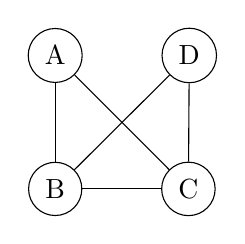
\begin{tikzpicture}
            \node[circle,draw] (a)               {A};
            \node[circle,draw] (b) [below = of a] {B};
            \node[circle,draw] (c) [right = of b] {C};
            \node[circle,draw] (d) [right = of a] {D};
            \path[-](a) edge      node {} (b)
                    (a) edge      node {} (c)
                    (b) edge      node {} (c)
                    (b) edge      node {} (d)
                    (c) edge      node {} (d);
        \end{tikzpicture}
        \caption{$ G_1 $}
        \label{fig:graph1}
    \end{minipage}
    \begin{minipage}[b]{0.5\textwidth}
        \centering
        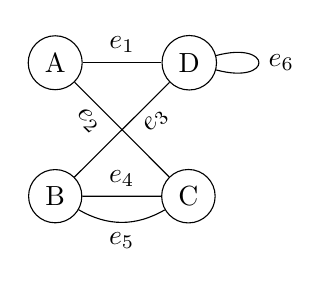
\begin{tikzpicture}[every loop/.style={},scale=1.5]
            \node[circle,draw] (a)               {A};
            \node[circle,draw] (b) [below = of a] {B};
            \node[circle,draw] (c) [right = of b] {C};
            \node[circle,draw] (d) [right = of a] {D};
            \path[-](a) edge             node[above] {$ e_1 $} (d)
                        edge             node[below left,sloped] {$e_2\;$} (c)
                    (b) edge             node[above] {$ e_4 $} (c)
                        edge             node[below right,sloped]{$\;e_3$} (d)
                        edge[bend right] node[below] {$ e_5 $} (c)
                    (d) edge[loop right] node[right] {$ e_6 $} ();
        \end{tikzpicture}
        \caption{$ G_2 $}
        \label{fig:graph2}
    \end{minipage}
\end{figure}
\section{Multigraphs} 
Look at the graph \ref{fig:graph2}, the edges $ e_4 $ and $ e_5 $ are called multiple edges since they connect the same endpoints and the edge $ e_6 $ is called a loop since its endpoints are the same vertex. Such a diagram is called multigraph.
\section{Degree}
The degree of a vertex $ v $ in a graph $ G $ written $ deg(v) $ is equal to the number of edges in $ G $ which contains $ v $, that is which are incident on $ v $. A vertex with degree zero is called isolated. In graph $ G_2 $, $ deg(D)=4,\,deg(C)=3 $.

A multigraph is said to be finite if it has a finite number of vertices and a finite number of edges. The finite graph with one vertex and no edges is called the trivial graph.
\section{Subgraph}
Consider a graph $ G=G(V,E) $. A graph $ H=H(V',E') $ is called a subgraph of $ G $ if the vertices and edges of $ H $ are contained in the vertices and edges of $ G $.
\section{Isomorphic Graphs and Homeomorphic Graph}
Graphs $ G(V,E) $ and $ G^*(V^*,E^*) $ are said to be homeomorphic if the can be obtained from the same graph or isomorphic graphs by dividing an edge with additional vertices.
\begin{figure}[H]
    \begin{minipage}[b]{.3\textwidth}
        \centering
        \begin{tikzpicture}
            \node[circle,draw](a){};
            \node[circle,draw](b)[above =of a]{};
            \node[circle,draw](c)[below =of a]{};
            \node[circle,draw](d)[left = of a]{};
            \node[circle,draw](e)[right =of a]{};
            \path[-](a) edge node{}(b)
                        edge node{}(c)
                        edge node{}(d)
                        edge node{}(e);
        \end{tikzpicture}
        \caption{Graph A}
        \label{fig:graphIsoA}
    \end{minipage}
    \begin{minipage}[b]{.3\textwidth}
        \centering
        \begin{tikzpicture}
            \node[circle,draw](a){};
            \node[circle,draw](b)[above =of a]{};
            \node[circle,draw](g)[above =of b]{};
            \node[circle,draw](f)[above =of g]{};
            \node[circle,draw](c)[below =of a]{};
            \node[circle,draw](d)[left = of a]{};
            \node[circle,draw](e)[right =of a]{};
            \path[-](a) edge node{}(b)
                        edge node{}(c)
                        edge node{}(d)
                        edge node{}(e)
                    (b) edge node{}(g)
                    (g) edge node{}(f);
        \end{tikzpicture}
        \caption{Graph B}
        \label{fig:graphIsoB}
    \end{minipage}
    \begin{minipage}[b]{.3\textwidth}
        \centering
        \begin{tikzpicture}
            \node[circle,draw](a){};
            \node[circle,draw](b)[above =of a]{};
            \node[circle,draw](f)[above =of b]{};
            \node[circle,draw](c)[below =of a]{};
            \node[circle,draw](g)[below =of c]{};
            \node[circle,draw](d)[left = of a]{};
            \node[circle,draw](e)[right =of a]{};
            \path[-](a) edge node{}(b)
                        edge node{}(c)
                        edge node{}(d)
                        edge node{}(e)
                    (b) edge node{}(f)
                    (c) edge node{}(g);
        \end{tikzpicture}
        \caption{Graph C}
        \label{fig:graphIsoC}
    \end{minipage}
\end{figure}
Graphs \ref{fig:graphIsoB} and \ref{fig:graphIsoC} are homeomorphic since they can be obtained from \ref{fig:graphIsoA} by adding appropriate vertices.

Graphs $ G $ and $ G^* $ are said to be isomorphic if there exists a one-to-one correspondence $ f:V\to V^* $ such that $ \set{u,v} $ is an edge of $ G $ if and only if $ \set{f(u),f(v)} $ is an edge of $ G^* $. 
\begin{figure}[H]
    \begin{minipage}[b]{.5\textwidth}
        \centering
        \begin{tikzpicture}
            \node[circle,draw] (a) {};
            \node[circle,draw] (c)[above right =of a] {};
            \node[circle,draw] (b)[below right =of c] {};
            \node[circle,draw] (d)[below left =of a] {};
            \node[circle,draw] (e)[below right =of b] {};
            \path[-] (a) edge node{} (b)
                        edge node{} (d)
                        edge node{} (c)
                    (b) edge node{} (c)
                        edge node{}(e);
            \node[node distance=.75cm](anchor)[right =of b]{};
            \node[circle,draw] (i)[right =of anchor] {};
            \node[circle,draw] (j)[above  =of i] {};
            \node[circle,draw,node distance=.25cm] (k)[right =of i] {};
            \node[circle,draw] (l)[below  =of i] {};
            \node[circle,draw] (m)[below right =of i] {};
            \path[-](i) edge node{}(j)
                        edge node{}(k)
                        edge node{}(l)
                    (k) edge[in=30, out=30] node{}(j)
                        edge node{}(m);
        
        \end{tikzpicture}
        \caption{Isomorphic Graphs}
        \label{fig:isoGraphA}
    \end{minipage}
    \begin{minipage}[b]{.5\textwidth}
        \centering
        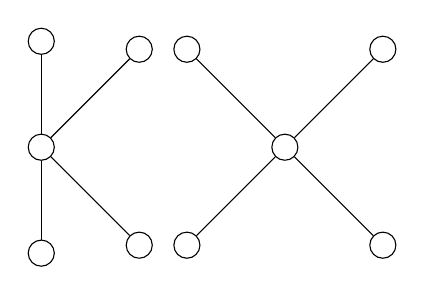
\begin{tikzpicture}
            \node[circle,draw] (a){};
            \node[circle,draw] (b)[above =of a]{};
            \node[circle,draw] (c)[below =of a]{};
            \node[circle,draw] (d)[above right =of a]{};
            \node[circle,draw] (e)[below right =of a]{};
            \path[-] (a) edge node{}(b)
                        edge node{}(c)
                        edge node{}(d)
                        edge node{}(e);
            \node[node distance=1.5cm](anchor)[right =of a]{};
            \node[circle,draw] (aa)[right =of anchor]{};
            \node[circle,draw] (bb)[above right =of aa]{};
            \node[circle,draw] (cc)[below right =of aa]{};
            \node[circle,draw] (dd)[above left =of aa]{};
            \node[circle,draw] (ee)[below left =of aa]{};
            \path[-] (aa) edge node{}(bb)
                        edge node{}(cc)
                        edge node{}(dd)
                        edge node{}(ee);
        \end{tikzpicture}
        \caption{Isomorphic Graphs}
        \label{fig:isoGraphB}
    \end{minipage}
\end{figure}
\section{Paths, Connectivity}
A path in a multigraph $ G $ consists of vertices and edges of the form,\\
\indent\indent $ v_0,\,e_1,\,v_1,\,e_1,\,v_2,\,e_2,\dots,\,e_{n-1},\,v_{n-1},\,e_n,\,v_n $.

Where each edge $ e_i $ contains the vertices $ v_{i-1} $ and $ v_i $. The number $ n $ of edges is called the length of the path.
\begin{itemize}
    \item The path is closed if $ v_0=v_n $.
    \item A simple path is a path in which all vertices are different.
    \item A path in which all edges are different will be called a trail.
    \item A cycle is a closed path in which all vertices are distinct except $ v_0=v_n $.\\
    \begin{center}
        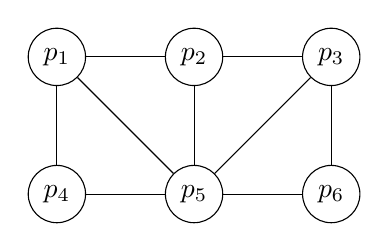
\begin{tikzpicture}
            \node[circle,draw] (a) {$ p_1 $};
            \node[circle,draw] (b)[right =of a] {$ p_2 $};
            \node[circle,draw] (c)[right =of b] {$ p_3 $};
            \node[circle,draw] (d)[below =of a] {$ p_4 $};
            \node[circle,draw] (e)[right =of d] {$ p_5 $};
            \node[circle,draw] (f)[right =of e] {$ p_6 $};
            \path[-](a) edge node{}(b)
                        edge node{}(d)
                        edge node{} (e)
                    (e) edge node{}(f)
                        edge node{}(b)
                        edge node{} (c)
                    (b) edge node{}(c)
                    (c) edge node {}(f)
                    (d) edge node {} (e);
        \end{tikzpicture}
    \end{center}
    $ \alpha=\set{p_4,p_1,p_2,p_5,p_1,p_2,p_3,p_6} $ is not a trail\\
    $ \beta=\set{p_4,p_1,p_5,p_2,p_6} $ is not a path\\
    $ \gamma=\set{p_4,p_1,p_5,p_2,p_3,p_5,p_6} $ is not a trail but not simple\\
    $ \delta=\set{p_4,p_1,p_5,p_3,p_6} $ is simple but not shortest\\
    \item A graph $ G $ is connected if there is a path between any two of its vertices.
    \item The distance between vertices $ u $ and $ v $ in $ G $ written $ d(u,v) $ is the length of the shortest path between $ u $ and $ v $ and the diameter of $ G $, written $ diam(g) $ is the maximum distance between any two points in $ G $.
    \begin{figure}[H]
        \begin{minipage}[b]{.5\textwidth}
            \centering
            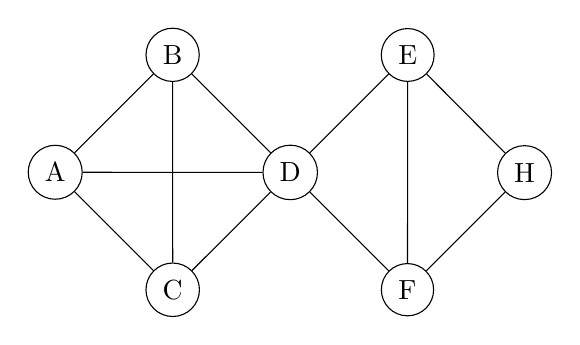
\begin{tikzpicture}
                \node[circle,draw] (a) {A};
                \node[circle,draw] (b)[above right=of a] {B};
                \node[circle,draw] (c)[below right=of a] {C};
                \node[circle,draw] (d)[below right=of b] {D};
                \node[circle,draw] (e)[above right=of d] {E};
                \node[circle,draw] (f)[below right=of d] {F};
                \node[circle,draw] (h)[above right=of f] {H};
                \path[-](a) edge node {}(b)
                            edge node {}(c)
                            edge node {} (d)
                        (b) edge node {}(d)
                            edge node{}(c)
                        (c) edge node {}(d)
                        (d) edge node{} (e)
                            edge node{}(f)
                        (e) edge node{}(h)
                            edge node{}(f)
                        (f) edge node{}(h);
            \end{tikzpicture}
            \caption{$ G_1 $}
            \label{fig:multi1}
        \end{minipage}
        \begin{minipage}[b]{.5\textwidth}
            \centering
            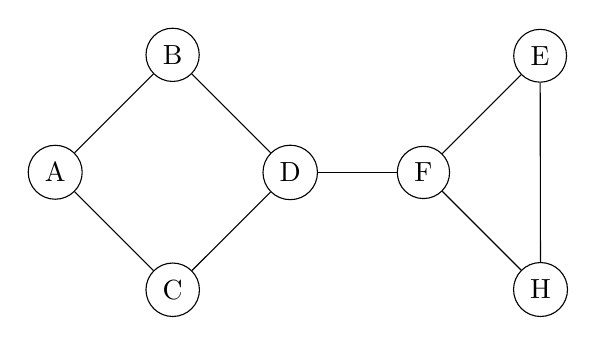
\begin{tikzpicture}
                \node[circle,draw] (a) {A};
                \node[circle,draw] (b)[above right=of a] {B};
                \node[circle,draw] (c)[below right=of a] {C};
                \node[circle,draw] (d)[below right=of b] {D};
                \node[circle,draw] (f)[right=of d] {F};
                \node[circle,draw] (e)[above right=of f] {E};
                \node[circle,draw] (h)[below right=of f] {H};
                \path[-](a) edge node {}(b)
                            edge node {}(c)
                        (b) edge node {}(d)
                        (c) edge node {}(d)
                        (d) edge node{} (f)
                        (f) edge node{}(h)
                            edge node{}(e)
                        (e) edge node{}(h);
            \end{tikzpicture}
            \caption{$ G_2 $}
            \label{fig:multi2}
        \end{minipage}
    \end{figure}
    In $ G_1 $(figure \ref{fig:multi1}), $ d(A,\,F)=2 $ and $ diam(G_1)=3 $\\
    In $ G_2 $(figure \ref{fig:multi2}), $ d(A,\,F)=3 $ and $ diam(G_2)=4 $
    \item A vertex $ v $ in $ G $ is called a cutpoint if $ G-v $ is disconnected.
    \item An edge $ e $ is called a bridge if $ G-e $ is disconnected.\\($ D $ in graph $ G_1 $ is cutpoint and $ e=\set{D,F} $ is a bridge in $ G_2 $.)
    \item  A multigraph is said to be traversable if it can be drawn without any breaks in the curve and without repeating any edges.\\
    \begin{center}
        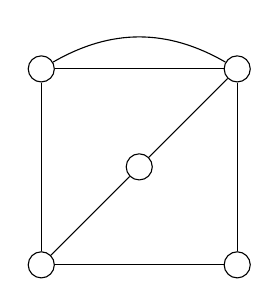
\begin{tikzpicture}
            \node[circle,draw] (a){};
            \node[circle,draw] (b)[below right=of a]{};
            \node[circle,draw] (c)[above right=of b]{};
            \node[circle,draw] (d)[below left=of b]{};
            \node[circle,draw] (e)[below right=of b]{};
            \path[-](a)edge node{}(c)
                    edge[bend left] node{}(c)
                    edge node{}(d)
                    (d) edge node{}(e)
                    edge node{}(b)
                    (e)edge node{}(c)
                    (c)edge node{}(b);
    
        \end{tikzpicture}\quad
        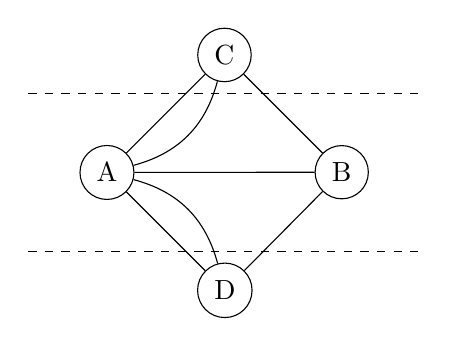
\begin{tikzpicture}
            \node[circle,draw](a){A};
            \node[circle,draw](c)[above right =of a]{C};
            \node[circle,draw](b)[below right =of c]{B};
            \node[circle,draw](d)[below right =of a]{D};
            \path[-](a) edge node{}(c)
                        edge [bend right] node {}(c)
                        edge node{}(b)
                        edge node{}(d)
                        edge[bend left] node {}(d)
                    (b)edge node{}(c)
                    edge node{}(d);
            \draw[dashed] (-1,1)--(4,1);
            \draw[dashed] (-1,-1)--(4,-1);
        \end{tikzpicture}
    \end{center}
    A multigraph with more than two odd vertices cannot be traversable. The famous k\"onigsberg bridge problem has four odd vertices.
    \item A graph $ G $ is called an Eulerian graph if there exists a closed traversable trail.
    \item A finite connected graph is Eulerian if and only if each vertex has even degree.
    \item A Hamiltonian circuit in a graph $ G $ named after the nineteenth-century Irish mathematician William Hamilton, is a closed path that visits every vertex in $ G $ exactly once.

    A graph $ G $ that admits a Hamiltonian circuit is called a Hamiltonian graph.
    \begin{figure}[h]
        \centering
        \begin{minipage}[b]{0.4\textwidth}
            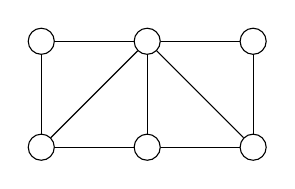
\begin{tikzpicture}
                \node[circle,draw](a){};
                \node[circle,draw](b)[right =of a]{};
                \node[circle,draw](c)[right =of b]{};
                \node[circle,draw](d)[below =of a]{};
                \node[circle,draw](e)[right =of d]{};
                \node[circle,draw](f)[right =of e]{};
                \path[-](b) edge node{}(a)
                            edge node{}(c)
                            edge node{}(d)
                            edge node{}(f)
                            edge node{}(e)
                        (a) edge node{}(d)
                        (e) edge node{}(d)
                            edge node{}(f)
                        (f) edge node{}(c);
            \end{tikzpicture}
            \caption{Hamiltonian and non-Eulerian}
            \label{fig:hamilNonEuler}
        \end{minipage}
        \begin{minipage}[b]{0.5\textwidth}
            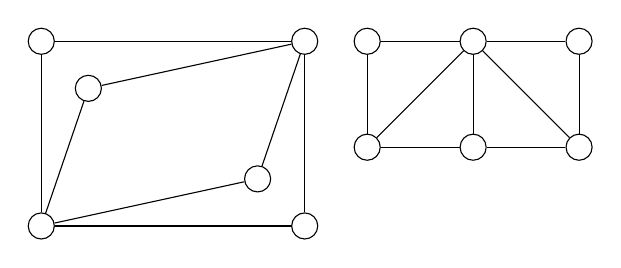
\begin{tikzpicture}
                \node[circle,draw](a){};
                \node[circle,draw, node distance = 3cm](b)[right =of a]{};
                \node[circle,draw, node distance =.5cm](c)[below right =of a]{};
                \node[circle,draw, node distance = 2cm](d)[below =of a]{};
    \node[circle,draw, node distance = 3cm](e)[right =of d]{};
    \node[circle,draw, node distance =.5cm](f)[above left =of e]{};
    \path[-](b) edge node{}(a)
                edge node{}(e)
                edge node{}(c)
                edge node{}(f)
            (d)edge node{}(a)
                edge node{}(e)
                edge node{}(c)
                edge node{}(f);
    \node[node distance=.1cm](anchor)[right=of b]{};
    \node[circle,draw,node distance=.1cm](aa)[right =of anchor]{};
    \node[circle,draw](bb)[right =of aa]{};
    \node[circle,draw](cc)[right =of bb]{};
    \node[circle,draw](dd)[below =of aa]{};
    \node[circle,draw](ee)[right =of dd]{};
    \node[circle,draw](ff)[right =of ee]{};
    \path[-](bb)edge node{}(aa)
                edge node{}(cc)
                edge node{}(dd)
                edge node{}(ff)
                edge node{}(ee)
            (dd)edge node{}(aa)
                edge node{}(ee)
            (ff)edge node{}(cc)
                edge node{}(ee);
            \end{tikzpicture}
            \caption{Eulerian and non-Hamilton}
            \label{fig:eulerNonHamil}
        \end{minipage}
    \end{figure}
    \item A graph $ G $ is called a labeled graph if its edges are assigned data of one kind.
    
    A graph $ G $ is called a weighted graph if each $ e $ of $ G $ is assigned a non-negative number $ w(e) $ called the weight or length of $ v $. 
    \item A graph $ G $ is said to be complete if every vertex in $ G $ is connected to every other vertex in $ G $. The complete graph with $ n $ vertices is denoted by $ k_n $.
    \begin{figure}[h]
        \centering
        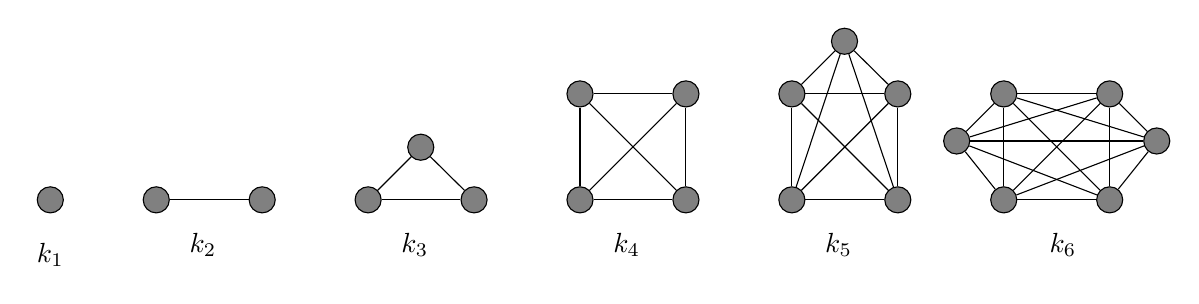
\begin{tikzpicture}
            [place/.style={circle,draw,fill=black!50}]
            \node[place] (a){};
            \node[node distance=.25cm] (text1)[below =of a]{$ k_1 $};
            \node[place] (b)[right=of a]{};
            \node[place] (c)[right=of b]{};
            \node[node distance=.25cm] (text2)[below right =of b]{$ k_2 $};
            \path[-](b)edge node{}(c);
            \node[place] (d)[right=of c]{};
            \node[place,node distance=.6cm] (e)[above right=of d]{};
            \node[place,node distance=1cm] (f)[right=of d]{};
            \node[node distance=.25cm] (text3)[below right =of d]{$ k_3 $};
            \path[-](e) edge node{}(d) edge node{}(f) (d)edge node{}(f);
            \node[place] (g)[right=of f]{};
            \node[place] (h)[right=of g]{};
            \node[place] (i)[above=of g]{};
            \node[place] (j)[right=of i]{};
            \node[node distance=.25cm] (text4)[below right =of g]{$ k_4 $};
            \path[-](g) edge node {} (i)
                        edge node {} (h)
                        edge node {} (j)
                    (i) edge node {} (j)
                        edge node {} (h)
                    (h) edge node {} (j);
            \node[place] (k)[right=of h]{};
            \node[place] (l)[right=of k]{};
            \node[place] (m)[above=of k]{};
            \node[place] (n)[right=of m]{};
            \node[place,node distance=.6cm] (o)[above right=of m]{};
            \node[node distance=.25cm] (text5)[below right =of k]{$ k_5 $};
            \path[-](k) edge node {} (m)
                        edge node {} (n)
                        edge node {} (l)
                        edge node {} (o)
                    (n) edge node {} (m)
                        edge node {} (l)
                        edge node {} (o)
                    (l) edge node {} (m)
                        edge node {} (o)
                    (m) edge node {} (o);
            
            \node[place] (q)[right=of l]{};
            \node[place] (r)[right=of q]{};
            \node[place] (s)[above=of q]{};
            \node[place] (t)[right=of s]{};
            \node[place,node distance=.5cm] (p)[below left=of s]{};
            \node[place,node distance=.5cm] (u)[below right=of t]{};
            \node[node distance=.25cm] (text6) [below left =of r]{$ k_6 $};
            \path[-](p) edge node {} (s)
                        edge node {} (q)
                        edge node {} (r)
                        edge node {} (t)
                        edge node {} (u)
                    (q) edge node {} (s)
                        edge node {} (r)
                        edge node {} (u)
                        edge node {} (t)
                    (t) edge node {} (s)
                        edge node {} (r)
                        edge node {} (u)
                    (s) edge node {} (r)
                        edge node {} (u)
                    (u) edge node {} (r);
        \end{tikzpicture}
        \caption{Some complete graphs}
        \label{fig:comGraph}
    \end{figure}
    \item A graph $ G $ is $ k $-regular if every vertex has degree $ k $.
    \begin{figure}[H]
        \centering
        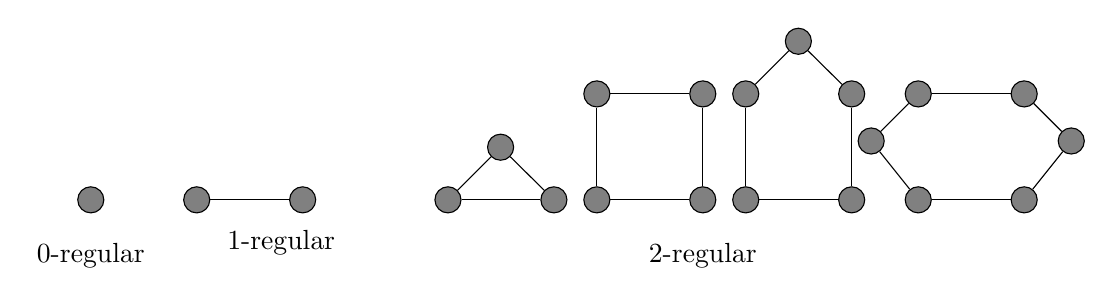
\begin{tikzpicture}
            [place/.style={circle,draw,fill=black!50}]
            \node[place] (a){};
            \node[node distance=.25cm] (text1)[below =of a]{0-regular};
            \node[place,node distance=1cm] (b)[right=of a]{};
            \node[place] (c)[right=of b]{};
            \node[node distance=.2cm] (text2)[below right=of b]{1-regular};
            \path[-](b)edge node{}(c);
            \node[place,node distance=1.5cm] (d)[right=of c]{};
            \node[place,node distance=.6cm] (e)[above right=of d]{};
            \node[place,node distance=1cm] (f)[right=of d]{};
            \path[-](e) edge node{}(d) edge node{}(f) (d)edge node{}(f);
            \node[place,node distance=.2cm] (g)[right=of f]{};
            \node[place] (h)[right=of g]{};
            \node[place] (i)[above=of g]{};
            \node[place] (j)[right=of i]{};
            \node[node distance=.25cm] (text4)[below =of h]{2-regular};
            \path[-](g) edge node {} (i)
                        edge node {} (h)
                    (i) edge node {} (j)
                    (h) edge node {} (j);
            \node[place,node distance=.2cm] (k)[right=of h]{};
            \node[place] (l)[right=of k]{};
            \node[place] (m)[above=of k]{};
            \node[place] (n)[right=of m]{};
            \node[place,node distance=.6cm] (o)[above right=of m]{};
            \path[-](k) edge node {} (m)
                        edge node {} (l)
                    (n) edge node {} (l)
                        edge node {} (o)
                    (m) edge node {} (o);
            
            \node[place,node distance=.5cm] (q)[right=of l]{};
            \node[place] (r)[right=of q]{};
            \node[place] (s)[above=of q]{};
            \node[place] (t)[right=of s]{};
            \node[place,node distance=.5cm] (p)[below left=of s]{};
            \node[place,node distance=.5cm] (u)[below right=of t]{};
            \path[-](p) edge node {} (s)
                        edge node {} (q)
                    (u) edge node {} (r)
                        edge node {} (t)
                    (t) edge node {} (s)
                    (r) edge node {} (q);
        \end{tikzpicture}
        \caption{Some regular graphs}
        \label{fig:regGraph}
    \end{figure}
    \item A graph $ G $ is said to be bipartite if its vertices $ V $ can be partitioned into two subsets $ M $ and $ N $ such that each edge of $ G $ connects a vertex of $ M $ to a vertex of $ N $.

    By $ k_{m,n} $ we mean that each vertex of $ M $ is connected to each vertex of $ N $, a complete bipartite graph.
    \begin{center}
        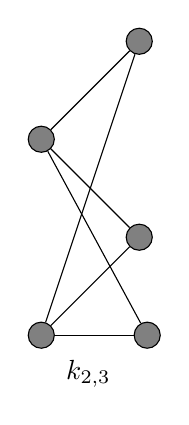
\begin{tikzpicture}
            [a/.style={circle,draw,fill=black!50}]
            \node[a](a) {};
            \node[a](b)[above right=of a] {};
            \node[a](c)[below right=of a] {};
            \node[a](d)[below left=of c] {};
            \node[a](e)[right=of d] {};
            \node[node distance=.1cm](text)[below right=of d] {$ k_{2,3} $};
            \path[-](a) edge node{}(b)edge node{}(c)edge node{}(e)
            (d)edge node{}(b)edge node{}(c)edge node{}(e);
        \end{tikzpicture}
    \end{center}
    \item A graph or multigraph which can be drawn in the plane so that its edges do not cross is said to be planar.
    \begin{center}
        \begin{tikzpicture}
            [place/.style={circle,draw}]
            \node[place] (g)[right=of f]{};
            \node[place] (h)[right=of g]{};
            \node[place] (i)[above=of g]{};
            \node[place] (j)[right=of i]{};
            \path[-](g) edge node {} (i)
                        edge node {} (h)
                        edge node {} (j)
                    (i) edge node {} (j)
                        edge node {} (h)
                    (h) edge node {} (j);
            \node[place,node distance=1.5cm] (gg)[right=of h]{};
            \node[place] (hh)[right=of gg]{};
            \node[place] (ii)[above=of gg]{};
            \node[place] (jj)[right=of ii]{};
            \path[-](gg) edge node {} (ii)
                        edge node {} (hh)
                        edge[in=120,out= 120,out looseness=3] node {} (jj)
                    (ii) edge node {} (jj)
                        edge node {} (hh)
                    (hh) edge node {} (jj);
        \end{tikzpicture}
    \end{center}
    \item A particular planar representation of a finite planar multigraph is called a map. 
    \item Let $ G $ be a connected planar graph with $ p $ vertices and $ q $ edges, where $ p\geq3 $. Then $ q\leq 3p-6 $.
    \item Suppose $ G $ is a graph with $ m $ vertices and suppose the vertices have been ordered say, $ v_1,v_2,\dots,v_m $. Then the adjacency matrix $ A=[a_{ij}] $ of the graph $ G $ is the $ m\times m $ matrix defined by \[a_{ij}=\begin{cases}
        1\quad\text{if $ v_i $ is adjacent to $ v_j $}\\
        0\quad\text{Otherwise}
    \end{cases}\]
    Adjacency matrix is symmetric.
    \begin{center}
        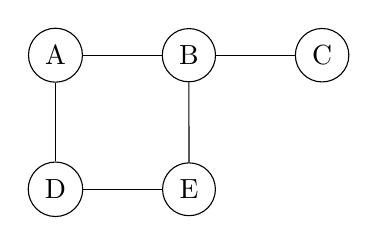
\begin{tikzpicture}
            [a/.style={circle,draw}]
            \node[a](a){A};
            \node[a](b)[right =of a]{B};
            \node[a](c)[right =of b]{C};
            \node[a](d)[below =of a]{D};
            \node[a](e)[right =of d]{E};
            \path[-](a) edge node{}(b)
                        edge node{}(d)
                    (e) edge node{}(d)
                        edge node{}(b)
                    (c) edge node{}(b);
        \end{tikzpicture}
        $ \bordermatrix{~ & A & B & C & D & E \cr
                        A & 0 & 1 & 0 & 1 & 0 \cr
                        B & 1 & 0 & 1 & 0 & 1 \cr
                        C & 0 & 1 & 0 & 0 & 0 \cr
                        D & 1 & 0 & 0 & 0 & 1 \cr
                        E & 0 & 1 & 0 & 1 & 0 \cr
                        } $
    \end{center}
    \item A vertex coloring or simply a coloring of $ G $ is an assignment of colors to the vertices of $ G $ such that adjacent vertices have different colors.

    The minimum number of colors needed to paint $ G $ is called the chromatic number of $ G $ and is denoted by $ \lambda(G) $.\\
    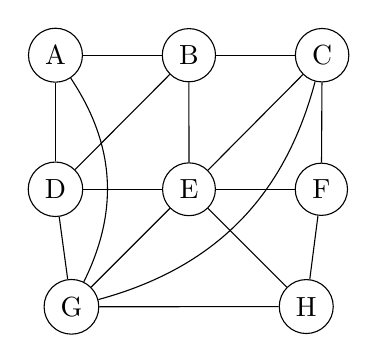
\begin{tikzpicture}
        [a/.style={circle,draw}]
        \node[a](a){A};
        \node[a](b)[right =of a]{B};
        \node[a](c)[right =of b]{C};
        \node[a](d)[below =of a]{D};
        \node[a](e)[right =of d]{E};
        \node[a](f)[right =of e]{F};
        \node[a](g)[below left =of e]{G};
        \node[a](h)[below right =of e]{H};
        \path[-](e) edge node{} (b)
                    edge node{} (c)
                    edge node{} (d)
                    edge node{} (f)
                    edge node{} (g)
                    edge node{} (h)
                (g) edge[bend right] node{} (a)
                    edge node{} (d)
                    edge node{} (h)
                    edge[bend right] node{} (c)
                (d) edge node{} (a)
                    edge node{} (b)
                (f) edge node{} (c)
                    edge node{} (h)
                (b) edge node{} (a)
                    edge node{} (c);
    \end{tikzpicture}
    \begin{enumerate}
        \item Ordering the vertices of $ G $ according to decreasing degrees. Here they are $ E,\,G,\,B,\,C,\,D,\,A,\,F,\,H $
        \item Assign first color $ c_1 $ to first vertex and assign $ c_1 $ to each vertex which is not adjacent to first vertex.
        \item Repeat step 2 with second color $ c_2 $.
        \item Repeat step 3 and 3 until no vertex left.
        \item Exit.
    \end{enumerate}
    First color $ c_1 $ to $ E,\,A $\\
    Second color $ c_2 $ to $ G, \,B,\,F $\\
    Third color $ c_3 $ to $ C,\,D,\,H $\\
    Since every vertex is adjacent to every other vertex, $ k_n $ requires $ n $ colors in any coloring. Thus $ \lambda(k_n)=n $.
\end{itemize}
\section{Four Color Theorem}
Any planar graph is four colorable.
\subsection{Dual maps and the four color theorem}
If the regions of any map $ M $ are colored so that adjacent regions have different colors, then no more than four colors are required.
Note to self:: TO BE ADDED
\section{Spanning Tree}
A subgraph $ T $ of a connected graph $ G $ is called a spanning tree of $ G $ if $ T $ is a tree and $ T $ includes all the vertices of $ G $.

Suppose $ G $ is a connected weighted graph. Then any spanning tree $ T $ of $ G $ is assigned a total weight obtained by adding the weights of the edges in $ T $.

A minimal spanning tree of $ G $ is a spanning tree whose total weight is as small as possible.
\subsection{Kruskal's algorithm for minimal spanning tree}
\begin{enumerate}[label=step \arabic*:]
    \item Arrange the edges of $ G $ in order of increasing weights.
    \item Starting only with the vertices of $ G $ and proceeding sequentially, add each edge which does not result in a cycle until $ (n-1) $ edges are added.
    \item Exit.
\end{enumerate}
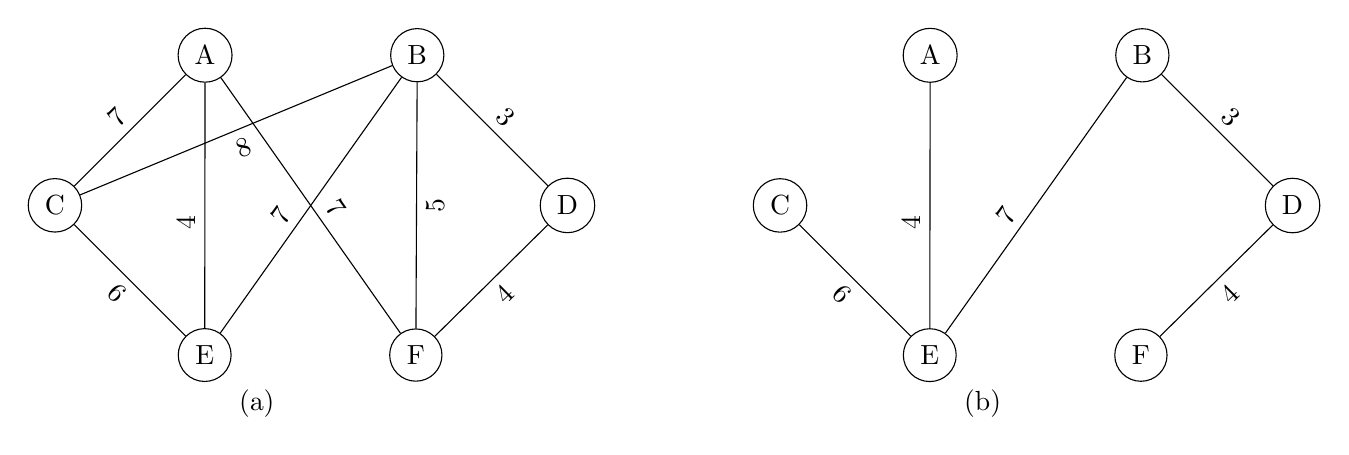
\begin{tikzpicture}
    [node distance=2cm,a/.style={circle,draw}]
    \node[a] (a) {A};
    \node[a] (b) [right =of a] {B};
    \node[a] (c) [below left =of a] {C};
    \node[a] (d) [below right =of b] {D};
    \node[a] (e) [below right =of c] {E};
    \node[a] (f) [right =of e] {F};
    \node[node distance=.1cm](text1)[below right=of e]{(a)};
    \path[-](a) edge node[above,sloped] {7}(c)
                edge node[above left,sloped] {4}(e)
                edge node[above right,sloped] {7}(f)
            (b) edge node[above left,sloped] {$ 7\,\, $}(e)
                edge node[below,sloped] {5}(f)
                edge node[above,sloped] {3}(d)
            (c) edge node[below,sloped] {8}(b)
                edge node[below,sloped] {6}(e)
            (d) edge node[below,sloped] {4}(f);
    
    \node[a] (cc) [right  =of d] {C};
    \node[a] (aa)[above right =of cc] {A};
    \node[a] (bb) [right =of aa] {B};
    \node[a] (dd) [below right =of bb] {D};
    \node[a] (ee) [below right =of cc] {E};
    \node[a] (ff) [right =of ee] {F};
    \node[node distance=.1cm](text2)[below right=of ee]{(b)};
    \path[-](aa)edge node[above left,sloped] {4}(ee)
            (bb) edge node[above left,sloped] {$ 7\,\, $}(ee)
                edge node[above,sloped] {3}(dd)
            (cc)edge node[below,sloped] {6}(ee)
            (dd)edge node[below,sloped] {4}(ff);
\end{tikzpicture}\\
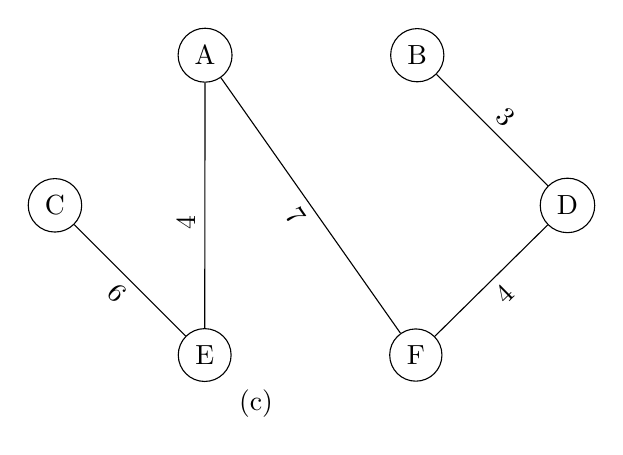
\begin{tikzpicture}
    [node distance=2cm,a/.style={circle,draw}]
    \node[a] (cc) {C};
    \node[a] (aa)[above right =of cc] {A};
    \node[a] (bb) [right =of aa] {B};
    \node[a] (dd) [below right =of bb] {D};
    \node[a] (ee) [below right =of cc] {E};
    \node[a] (ff) [right =of ee] {F};
    \node[node distance=.1cm](text1)[below right=of ee]{(c)};
    \path[-](aa)edge node[above left,sloped] {4}(ee)
                edge node[below,sloped] {7}(ff)
            (bb) edge node[above,sloped] {3}(dd)
            (cc)edge node[below,sloped] {6}(ee)
            (dd)edge node[below,sloped] {4}(ff);
\end{tikzpicture}\\
First we order the edges by decreasing weights and then we successively delete edges without disconnecting $ Q $ until five edges remain. This yields the following data:\\
\begin{tabular}{c c c c c c c c c c}
    Edges & BC & AF & AC & BE & CE & BF & AE & DF & BD \\
    Weight & 8 & 7 & 7 & 7 & 6 & 5 & 4 & 4 & 3\\
    Delete & Yes & Yes & Yes & No  & No & Yes & No & No & No\\
\end{tabular}\\
Thus the minimal spanning tree of $ Q $ which is obtained contains the edges \[BE,\,CE,\,AE,\,DF,\,BD\]
\section{Traversing Binary Tree}
There are three standard ways of traversing a binary tree $ T $ with root $ R $. these three algorithm called pre order, in order and post order.
\subsection{Pre order}
\begin{enumerate}
    \item Process the root $ R $.
    \item Traverse the left subtree of $ R $ in pre order.
    \item Traverse the right subtree of $ R $ in pre order.
\end{enumerate}
\subsection{In order}
\begin{enumerate}
    \item Traverse the left subtree of $ R $ in in order.
    \item Process the root $ R $.
    \item Traverse the right subtree of $ R $ in in order.
\end{enumerate}
\subsection{Post order}
\begin{enumerate}
    \item Traverse the left subtree of $ R $ in post order.
    \item Traverse the right subtree of $ R $ in post order.
    \item Process the root $ R $.
\end{enumerate}
\begin{ex}
    Traverse the tree of the following figure.\\
    \begin{tikzpicture}
        [level/.style={sibling distance = 5cm/#1,level distance = 1.5cm}]
        \node[]{A}
        child{node[] {B}
            child{node[]{D}}
            child{node[]{E}
                child{node[]{F}}
                child[missing]
            }
        }
        child{node[]{C}
            child{node[]{G}}
            child{node[]{H}
                child{node[]{J}
                    child{node[]{L}}
                    child[missing]
                }
                child{node[]{K}}
            }
        };
    \end{tikzpicture}
    \\
    Preorder traversal = $ A,\,B,\,D,\,E,\,F,\,C,\,G,\,H,\,J,\,L,\,K $\\
    Inorder traversal = $ D,\,B,\,F,\,E,\,A,\,G,\,C,\,L,\,J,\,H,\,K $\\
    Postorder traversal = $ D,\,F,\,E,\,B,\,G,\,L,\,J,\,K,\,H,\,C,\,A $ 
\end{ex}
\begin{ex}
    Using Dijkstra's algorithm to find shortest path from $ a $ to $ z $.\\
    \begin{enumerate}[label=step \arabic*:]
        \item \hfill
        \begin{figure}[H]
            \centering
            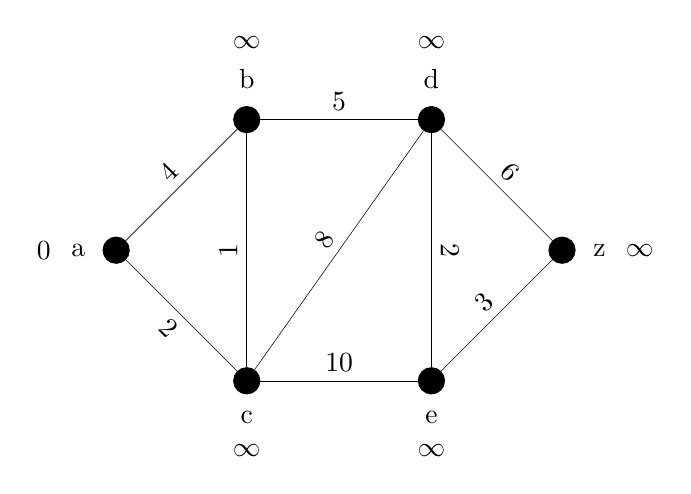
\begin{tikzpicture}
                [n/.style={circle,draw},node distance=2cm,
                dot/.style={circle,draw,fill=black,minimum size=1pt}]
                \node[dot] (a){};
                \node[node distance=1mm] (texta)[left=of a]{a};
                \node[node distance=.1mm] (textaa)[left=of texta]{0};
                \node[dot](b)[above right=of a]{};
                \node[node distance=1mm] (textb)[above=of b]{b};
                \node[node distance=.1mm] (textbb)[above=of textb]{$ \infty $};
                \node[dot](c)[below right=of a]{};
                \node[node distance=1mm] (textc)[below=of c]{c};
                \node[node distance=.1mm] (textcc)[below=of textc]{$ \infty $};
                \node[dot](d)[right=of b]{};
                \node[node distance=1mm] (textd)[above=of d]{d};
                \node[node distance=.1mm] (textdd)[above=of textd]{$ \infty $};
                \node[dot](e)[right=of c]{};
                \node[node distance=1mm] (texte)[below=of e]{e};
                \node[node distance=.1mm] (textee)[below=of texte]{$ \infty $};
                \node[dot](z)[above right=of e]{};
                \node[node distance=1mm] (textz)[right=of z]{z};
                \node[node distance=.1mm] (textzz)[right=of textz]{$ \infty $};
                \path[-](c) edge[very thin] node[above,sloped]{1}(b)
                            edge[very thin] node[below,sloped]{2}(a)
                            edge[very thin] node[above,sloped]{8}(d)
                            edge[very thin] node[above,sloped]{10}(e)
                        (b) edge[very thin] node[above,sloped]{4}(a)
                            edge[very thin] node[above,sloped]{5}(d)
                        (z) edge[very thin] node[above,sloped]{6}(d)
                            edge[very thin] node[above,sloped]{3}(e)
                        (d) edge[very thin] node[above,sloped]{2}(e);
            \end{tikzpicture}
        \end{figure}
        \item \hfill\begin{center}
            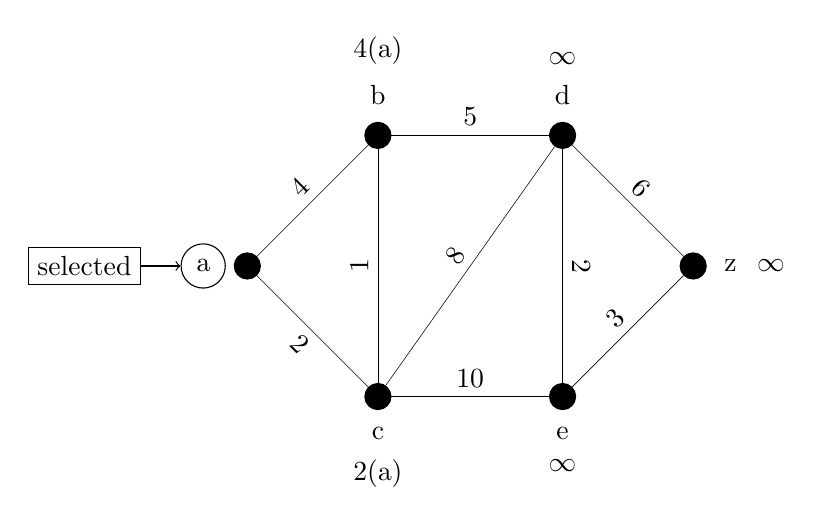
\begin{tikzpicture}
                [n/.style={circle,draw},node distance=2cm,
                dot/.style={circle,draw,fill=black,minimum size=1pt}]
                \node[dot] (a){};
                \node[n,node distance=1mm] (texta)[left=of a]{a};
                \node[rectangle,draw,node distance=5mm] (textaa)[left=of texta]{selected};
                \path[->](textaa)edge node{}(texta);
                \node[dot](b)[above right=of a]{};
                \node[node distance=1mm] (textb)[above=of b]{b};
                \node[node distance=.1mm] (textbb)[above=of textb]{4(a)};
                \node[dot](c)[below right=of a]{};
                \node[node distance=1mm] (textc)[below=of c]{c};
                \node[node distance=.1mm] (textcc)[below=of textc]{2(a)};
                \node[dot](d)[right=of b]{};
                \node[node distance=1mm] (textd)[above=of d]{d};
                \node[node distance=.1mm] (textdd)[above=of textd]{$ \infty $};
                \node[dot](e)[right=of c]{};
                \node[node distance=1mm] (texte)[below=of e]{e};
                \node[node distance=.1mm] (textee)[below=of texte]{$ \infty $};
                \node[dot](z)[above right=of e]{};
                \node[node distance=1mm] (textz)[right=of z]{z};
                \node[node distance=.1mm] (textzz)[right=of textz]{$ \infty $};
                \path[-](c) edge[very thin] node[above,sloped]{1}(b)
                            edge[very thin] node[below,sloped]{2}(a)
                            edge[very thin] node[above,sloped]{8}(d)
                            edge[very thin] node[above,sloped]{10}(e)
                        (b) edge[very thin] node[above,sloped]{4}(a)
                            edge[very thin] node[above,sloped]{5}(d)
                        (z) edge[very thin] node[above,sloped]{6}(d)
                            edge[very thin] node[above,sloped]{3}(e)
                        (d) edge[very thin] node[above,sloped]{2}(e);
            \end{tikzpicture}
        \end{center}
        \item \hfill\begin{center}
            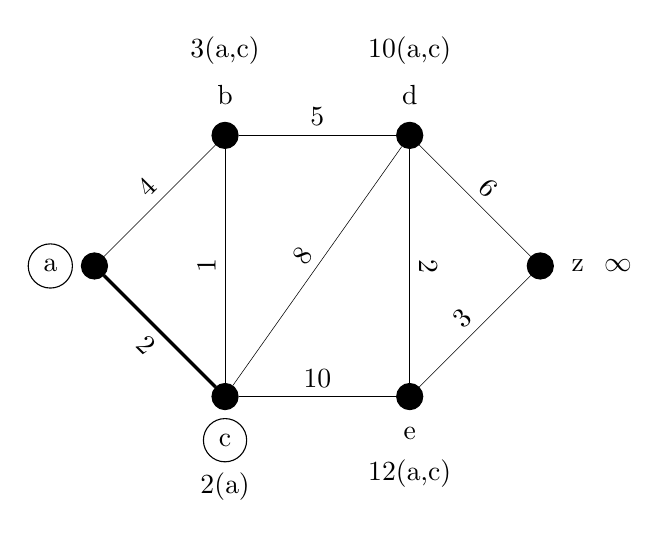
\begin{tikzpicture}
                [n/.style={circle,draw},node distance=2cm,
                dot/.style={circle,draw,fill=black,minimum size=1pt}]
                \node[dot] (a){};
                \node[n,node distance=1mm] (texta)[left=of a]{a};
                % \node[node distance=.1mm] (textaa)[left=of texta]{0};
                \node[dot](b)[above right=of a]{};
                \node[node distance=1mm] (textb)[above=of b]{b};
                \node[node distance=.1mm] (textbb)[above=of textb]{3(a,c)};
                \node[dot](c)[below right=of a]{};
                \node[n,node distance=1mm] (textc)[below=of c]{c};
                \node[node distance=.1mm] (textcc)[below=of textc]{2(a)};
                \node[dot](d)[right=of b]{};
                \node[node distance=1mm] (textd)[above=of d]{d};
                \node[node distance=.1mm] (textdd)[above=of textd]{10(a,c)};
                \node[dot](e)[right=of c]{};
                \node[node distance=1mm] (texte)[below=of e]{e};
                \node[node distance=.1mm] (textee)[below=of texte]{12(a,c)};
                \node[dot](z)[above right=of e]{};
                \node[node distance=1mm] (textz)[right=of z]{z};
                \node[node distance=.1mm] (textzz)[right=of textz]{$ \infty $};
                \path[-](c) edge[very thin] node[above,sloped]{1}(b)
                            edge[very thick] node[below,sloped]{2}(a)    
                            edge[very thin] node[above,sloped]{8}(d)
                            edge[very thin] node[above,sloped]{10}(e)
                        (b) edge[very thin] node[above,sloped]{4}(a)
                            edge[very thin] node[above,sloped]{5}(d)
                        (z) edge[very thin] node[above,sloped]{6}(d)
                            edge[very thin] node[above,sloped]{3}(e)
                        (d) edge[very thin] node[above,sloped]{2}(e);
            \end{tikzpicture}
        \end{center}
        \item \hfill\begin{center}
            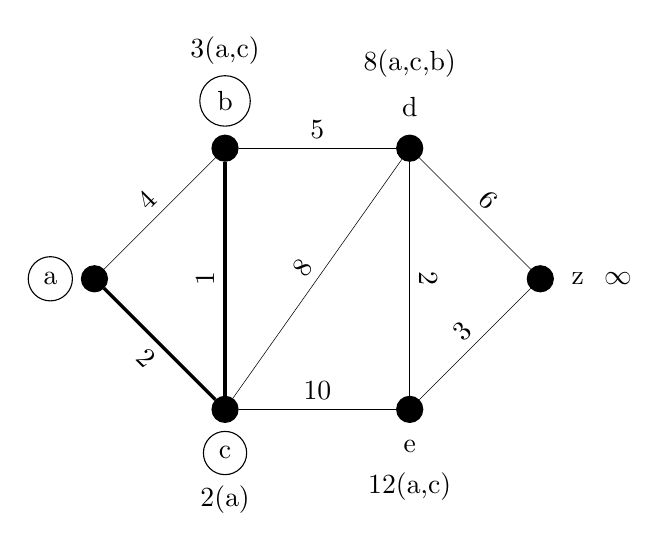
\begin{tikzpicture}
                [n/.style={circle,draw},node distance=2cm,
                dot/.style={circle,draw,fill=black,minimum size=1pt}]
                \node[dot] (a){};
                \node[n,node distance=1mm] (texta)[left=of a]{a};
                % \node[node distance=.1mm] (textaa)[left=of texta]{0};
                \node[dot](b)[above right=of a]{};
                \node[n,node distance=1mm] (textb)[above=of b]{b};
                \node[node distance=.1mm] (textbb)[above=of textb]{3(a,c)};
                \node[dot](c)[below right=of a]{};
                \node[n,node distance=1mm] (textc)[below=of c]{c};
                \node[node distance=.1mm] (textcc)[below=of textc]{2(a)};
                \node[dot](d)[right=of b]{};
                \node[node distance=1mm] (textd)[above=of d]{d};
                \node[node distance=.1mm] (textdd)[above=of textd]{8(a,c,b)};
                \node[dot](e)[right=of c]{};
                \node[node distance=1mm] (texte)[below=of e]{e};
                \node[node distance=.1mm] (textee)[below=of texte]{12(a,c)};
                \node[dot](z)[above right=of e]{};
                \node[node distance=1mm] (textz)[right=of z]{z};
                \node[node distance=.1mm] (textzz)[right=of textz]{$ \infty $};
                \path[-](c) edge[very thick] node[above,sloped]{1}(b)
                            edge[very thick] node[below,sloped]{2}(a)
                            edge[very thin] node[above,sloped]{8}(d)
                            edge[very thin] node[above,sloped]{10}(e)
                        (b) edge[very thin] node[above,sloped]{4}(a)
                            edge[very thin] node[above,sloped]{5}(d)
                        (z) edge[very thin] node[above,sloped]{6}(d)
                            edge[very thin] node[above,sloped]{3}(e)
                        (d) edge[very thin] node[above,sloped]{2}(e);
            \end{tikzpicture}
        \end{center}
        \item \hfill\begin{center}
            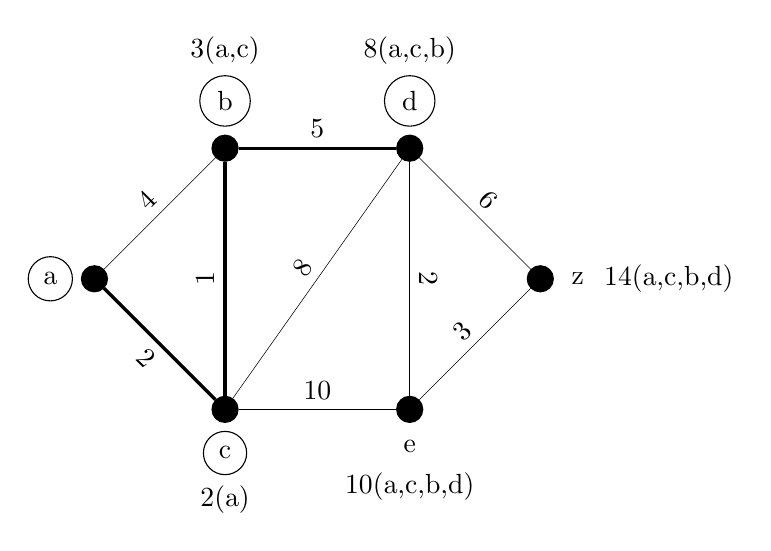
\begin{tikzpicture}
                [n/.style={circle,draw},node distance=2cm,
                dot/.style={circle,draw,fill=black,minimum size=1pt}]
                \node[dot] (a){};
                \node[n,node distance=1mm] (texta)[left=of a]{a};
                % \node[node distance=.1mm] (textaa)[left=of texta]{0};
                \node[dot](b)[above right=of a]{};
                \node[n,node distance=1mm] (textb)[above=of b]{b};
                \node[node distance=.1mm] (textbb)[above=of textb]{3(a,c)};
                \node[dot](c)[below right=of a]{};
                \node[n,node distance=1mm] (textc)[below=of c]{c};
                \node[node distance=.1mm] (textcc)[below=of textc]{2(a)};
                \node[dot](d)[right=of b]{};
                \node[n,node distance=1mm] (textd)[above=of d]{d};
                \node[node distance=.1mm] (textdd)[above=of textd]{8(a,c,b)};
                \node[dot](e)[right=of c]{};
                \node[node distance=1mm] (texte)[below=of e]{e};
                \node[node distance=.1mm] (textee)[below=of texte]{10(a,c,b,d)};
                \node[dot](z)[above right=of e]{};
                \node[node distance=1mm] (textz)[right=of z]{z};
                \node[node distance=.1mm] (textzz)[right=of textz]{14(a,c,b,d)};
                \path[-](c) edge[very thick] node[above,sloped]{1}(b)
                            edge[very thick] node[below,sloped]{2}(a)
                            edge[very thin] node[above,sloped]{8}(d)
                            edge[very thin] node[above,sloped]{10}(e)
                        (b) edge[very thin] node[above,sloped]{4}(a)
                            edge[very thick] node[above,sloped]{5}(d)
                        (z) edge[very thin] node[above,sloped]{6}(d)
                            edge[very thin] node[above,sloped]{3}(e)
                        (d) edge[very thin] node[above,sloped]{2}(e);
            \end{tikzpicture}
        \end{center}
        \item \hfill\begin{center}
            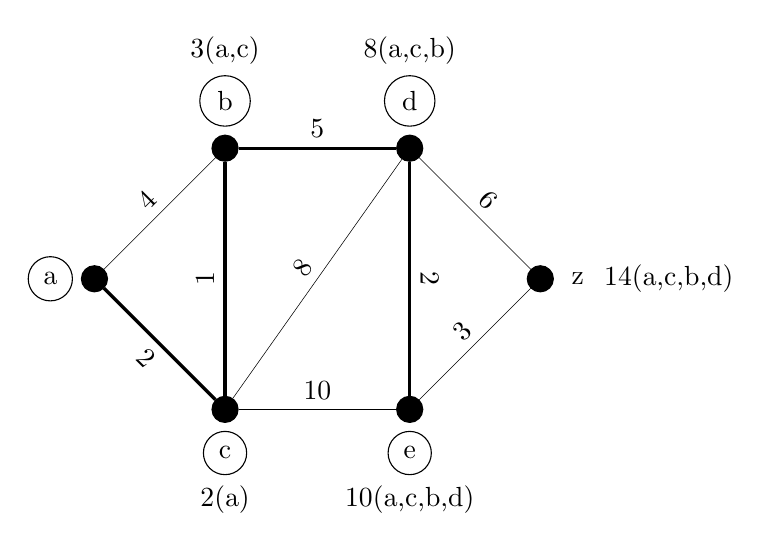
\begin{tikzpicture}
                [n/.style={circle,draw},node distance=2cm,
                dot/.style={circle,draw,fill=black,minimum size=1pt}]
                \node[dot] (a){};
                \node[n,node distance=1mm] (texta)[left=of a]{a};
                % \node[node distance=.1mm] (textaa)[left=of texta]{0};
                \node[dot](b)[above right=of a]{};
                \node[n,node distance=1mm] (textb)[above=of b]{b};
                \node[node distance=.1mm] (textbb)[above=of textb]{3(a,c)};
                \node[dot](c)[below right=of a]{};
                \node[n,node distance=1mm] (textc)[below=of c]{c};
                \node[node distance=.1mm] (textcc)[below=of textc]{2(a)};
                \node[dot](d)[right=of b]{};
                \node[n,node distance=1mm] (textd)[above=of d]{d};
                \node[node distance=.1mm] (textdd)[above=of textd]{8(a,c,b)};
                \node[dot](e)[right=of c]{};
                \node[n,node distance=1mm] (texte)[below=of e]{e};
                \node[node distance=.1mm] (textee)[below=of texte]{10(a,c,b,d)};
                \node[dot](z)[above right=of e]{};
                \node[node distance=1mm] (textz)[right=of z]{z};
                \node[node distance=.1mm] (textzz)[right=of textz]{14(a,c,b,d)};
                \path[-](c) edge[very thick] node[above,sloped]{1}(b)
                            edge[very thick] node[below,sloped]{2}(a)
                            edge[very thin] node[above,sloped]{8}(d)
                            edge[very thin] node[above,sloped]{10}(e)
                        (b) edge[very thin] node[above,sloped]{4}(a)
                            edge[very thick] node[above,sloped]{5}(d)
                        (z) edge[very thin] node[above,sloped]{6}(d)
                            edge[very thin] node[above,sloped]{3}(e)
                        (d) edge[very thick] node[above,sloped]{2}(e);
            \end{tikzpicture}
        \end{center}
        \item \hfill\begin{center}
            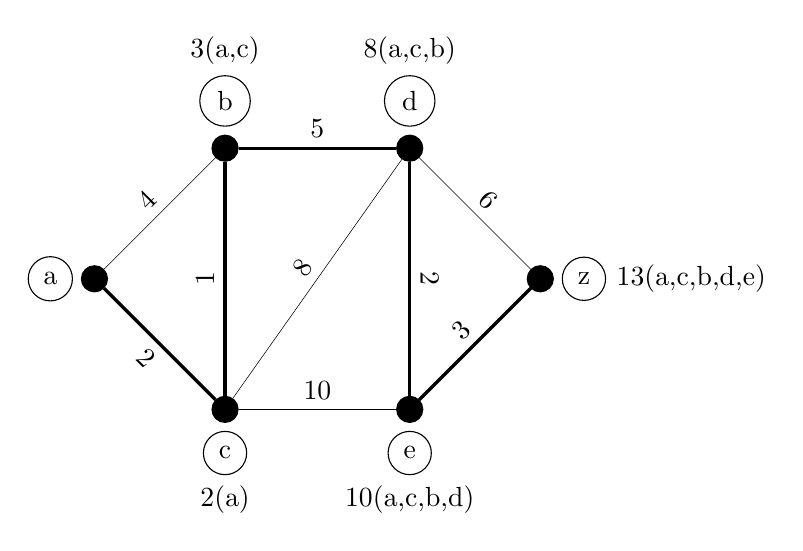
\begin{tikzpicture}
                [n/.style={circle,draw},node distance=2cm,
                dot/.style={circle,draw,fill=black,minimum size=1pt}]
                \node[dot] (a){};
                \node[n,node distance=1mm] (texta)[left=of a]{a};
                % \node[node distance=.1mm] (textaa)[left=of texta]{0};
                \node[dot](b)[above right=of a]{};
                \node[n,node distance=1mm] (textb)[above=of b]{b};
                \node[node distance=.1mm] (textbb)[above=of textb]{3(a,c)};
                \node[dot](c)[below right=of a]{};
                \node[n,node distance=1mm] (textc)[below=of c]{c};
                \node[node distance=.1mm] (textcc)[below=of textc]{2(a)};
                \node[dot](d)[right=of b]{};
                \node[n,node distance=1mm] (textd)[above=of d]{d};
                \node[node distance=.1mm] (textdd)[above=of textd]{8(a,c,b)};
                \node[dot](e)[right=of c]{};
                \node[n,node distance=1mm] (texte)[below=of e]{e};
                \node[node distance=.1mm] (textee)[below=of texte]{10(a,c,b,d)};
                \node[dot](z)[above right=of e]{};
                \node[n,node distance=1mm] (textz)[right=of z]{z};
                \node[node distance=.1mm] (textzz)[right=of textz]{13(a,c,b,d,e)};
                \path[-](c) edge[very thick] node[above,sloped]{1}(b)
                            edge[very thick] node[below,sloped]{2}(a)
                            edge[very thin] node[above,sloped]{8}(d)
                            edge[very thin] node[above,sloped]{10}(e)
                        (b) edge[very thin] node[above,sloped]{4}(a)
                            edge[very thick] node[above,sloped]{5}(d)
                        (z) edge[very thin] node[above,sloped]{6}(d)
                            edge[very thick] node[above,sloped]{3}(e)
                        (d) edge[very thick] node[above,sloped]{2}(e);
            \end{tikzpicture}
        \end{center}
    \end{enumerate}
    The shortest path: $ a\to c\to b\to d\to e\to z $
\end{ex}
\section{Graphical Representation of an Expression}
In compiler construction an expression such as $ '(x-y)*(w+z)*(x-y)*(w-z)' $ can be represented by the directed acyclic graph\footnote{See tree traversal, infix postfix expression, expression tree.}.
\begin{center}
    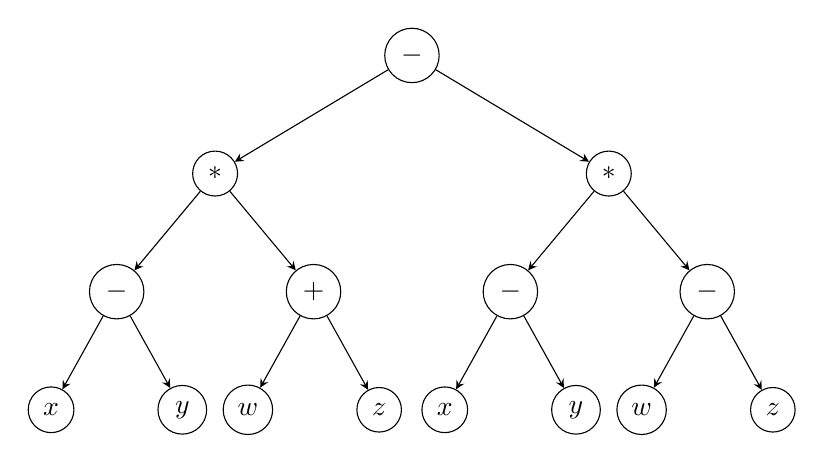
\begin{tikzpicture}
        [->,>=stealth,
        level/.style={sibling distance = 5cm/#1,level distance = 1.5cm},
        a/.style={text centered,align=center,circle,draw}]
        \node[a]{$ - $}
        child{node[a] {$ * $}
            child{node[a]{$ - $}
                child{node[a]{$ x $}}
                child{node[a]{$ y $}}
            }
            child{node[a]{$ + $}
                child{node[a]{$ w $}}
                child{node[a]{$ z $}}
            }
        }
        child{node[a]{$ * $}
            child{node[a]{$ - $}
                child{node[a]{$ x $}}
                child{node[a]{$ y $}}
            }
            child{node[a]{$ - $}
                child{node[a]{$ w $}}
                child{node[a]{$ z $}}
            }
        };
    \end{tikzpicture}
\end{center}
\begin{ex}
    Draw the tree which corresponds to the expression $ E=(2x+y)(5a-b)^3 $\\
    \begin{center}
        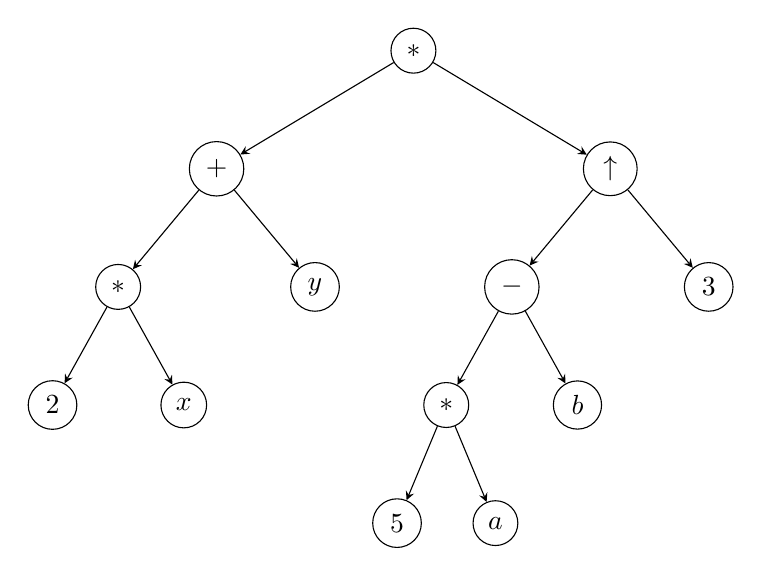
\begin{tikzpicture}
            [->,>=stealth,
            level/.style={sibling distance = 5cm/#1,level distance = 1.5cm},
            a/.style={text centered,align=center,circle,draw}]
            \node[a]{$ * $}
            child{node[a] {$ + $}
                child{node[a]{$ * $}
                    child{node[a]{$ 2 $}}
                    child{node[a]{$ x $}}
                }
                child{node[a]{$ y $}
                    % child{node[a]{$ w $}}
                    % child{node[a]{$ z $}}
                }
            }
            child{node[a]{$ \uparrow $}
                child{node[a]{$ - $}
                    child{node[a]{$ * $}
                        child{node[a]{$ 5 $}}
                        child{node[a]{$ a $}}
                    }
                    child{node[a]{$ b $}}
                }
                child{node[a]{$ 3 $}
                    % child{node[a]{$ w $}}
                    % child{node[a]{$ z $}}
                }
            };
        \end{tikzpicture}
    \end{center}
\end{ex}
\end{document}